\documentclass{article}
\usepackage{listings}
\usepackage{xcolor}

\definecolor{codegreen}{rgb}{0,0.6,0}
\definecolor{codegray}{rgb}{0.5,0.5,0.5}
\definecolor{codepurple}{rgb}{0.58,0,0.82}
\definecolor{backcolour}{rgb}{0.95,0.95,0.92}

\lstdefinestyle{mystyle}{
    backgroundcolor=\color{backcolour},   
    commentstyle=\color{codegreen},
    keywordstyle=\color{magenta},
    numberstyle=\tiny\color{codegray},
    stringstyle=\color{codepurple},
    basicstyle=\ttfamily\footnotesize,
    breakatwhitespace=false,         
    breaklines=true,                 
    captionpos=b,                    
    keepspaces=true,                 
    numbers=left,                    
    numbersep=5pt,                  
    showspaces=false,                
    showstringspaces=false,
    showtabs=false,                  
    tabsize=2
}

\lstset{style=mystyle}
\usepackage{hcmut-report}
\usepackage{codespace}

\usepackage{courier} %% Sets font for listing as Courier.
\lstset{
tabsize = 4, %% set tab space width
showstringspaces = false, %% prevent space marking in strings, string is defined as the text that is generally printed directly to the console
numbers = left, %% display line numbers on the left
commentstyle = \color{green}, %% set comment color
keywordstyle = \color{blue}, %% set keyword color
stringstyle = \color{red}, %% set string color
rulecolor = \color{black}, %% set frame color to avoid being affected by text color
basicstyle = \small \ttfamily , %% set listing font and size
breaklines = true, %% enable line breaking
numberstyle = \tiny,
}


% Sub-preambles
% https://github.com/MartinScharrer/standalone
% Encodings
\usepackage{amsmath,amssymb,gensymb,textcomp}

% Better tables
% Wide tables go to https://tex.stackexchange.com/q/332902
\usepackage{array,multicol,multirow,siunitx,tabularx}

% Better enum
\usepackage{enumitem}

% Graphics
\usepackage{caption,float}

% Allow setting >max< width of figure
% Remove if unneeded
\usepackage[export]{adjustbox} % 'export' allows adjustbox keys in \includegraphics
\usepackage{mwe}

% Custom commands
% Remove if unneeded
\newcommand*\mean[1]{\bar{#1}}

\ocoursename{CO3091 - LOGIC DESIGN PROJECT}
\oreporttype{ASSIGNMENT REPORT}
\title{\huge{FOUR-WAY TRAFFIC LIGHT}}
\oinstructor{PROF. NGUYEN CAO TRI}

\reportlayout%

\begin{document}

\coverpage%
\section*{Member list}
\begin{center}
  \begin{tabular}{>{\stepcounter{memberrowno}\thememberrowno}llcc}
    \toprule
    \multicolumn{1}{c}{\textbf{No.}} & \textbf{Full name} & \textbf{Student ID}\\
    \midrule
                                1     & Nguyen Khanh Nam                  &2153599                \\
                                2     & Nguyen Vu Khanh                     & 2153444                \\
    \bottomrule
  \end{tabular}
\end{center}

\newpage
\tableofcontents

\newpage

\section{Introduction}
In the realm of traffic management, the quest for efficient and innovative solutions has led to the exploration of logic design principles in creating a four-way traffic control system. This project delves into the conceptualization, design, and implementation of a traffic control mechanism devoid of conventional technologies. By leveraging the capabilities of specific integrated circuits (ICs) such as SN74LS175N, SN74LS193N, and CD4511BE, the aim was to engineer a traffic control system that operates seamlessly, adheres to predefined sequences, and allows for manual intervention when necessary.

The project introduces two fundamental modes of operation: Automatic and Manual. In the Automatic Mode, the system follows a predetermined sequence, ensuring optimal traffic flow through accurate signal timing. Conversely, the Manual Mode provides a dynamic element, empowering authorities to manually control traffic signals in response to specific situations, such as traffic congestion.

To complement the functionality of the system, a 7-segment display, driven by CD4017BE, was incorporated. This display serves as a visual representation of the countdown sequence, providing a clear and intuitive indication of the changing traffic signal states.

This report outlines the entire process of designing, implementing, and simulating the four-way traffic control system. Through a combination of logic design principles and strategic use of ICs, the project aims to showcase the viability and efficacy of a logic-based approach in the realm of traffic management.

\begin{figure}[h]
    \centering
    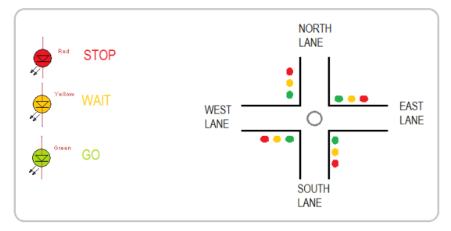
\includegraphics[width=12cm]{Pic/Pictures/4 ways.png}
    \caption{Four-way traffic problem.}
    \label{fig:enter-label}
\end{figure}
\newpage

\section{Theoretical Basis}
\subsection{How NE555 Module Work}
The NE555, or simply 555 timer IC, is an integrated circuit that can be used as a versatile timer or pulse generator. It operates in three modes: \textbf{monostable}, \textbf{astable}, and \textbf{bistable}. The most common modes are monostable and astable.\par
\subsubsection{Monostable Mode}\par
\begin{itemize}
    \item In monostable mode, the 555 acts as a one-shot pulse generator.
    \item When triggered (pin 2, TRIG, is brought below 1/3 of Vcc), the 555 produces a single, fixed-width pulse.
    \item The width of the pulse is determined by an external resistor (R) and capacitor (C) connected to pins 6 (THR) and 2 (TRIG).
\end{itemize}

\vspace{10pt}
\textbf{The pulse width (t)} is given by the equation: $t = 1.1 \times R \times C$.\par
\textbf{The time constant ($\tau$)} is given by: $\tau = R \times C$.\par
\vspace{10pt}
\textbf{Operation Steps:}

\begin{itemize}
    \item Upon trigger, the internal flip-flop is set, and the output (pin 3, OUT) goes high.
    \item The capacitor (C) charges through resistor R.
    \item When the voltage across C reaches 2/3 of Vcc, the flip-flop resets, and the output goes low.
    \item The capacitor discharges through an external discharge transistor.
\end{itemize}

\vspace{10pt}

\textbf{Applications:} Monostable mode is often used for generating precise time delays.

\begin{figure}[h]
    \centering
    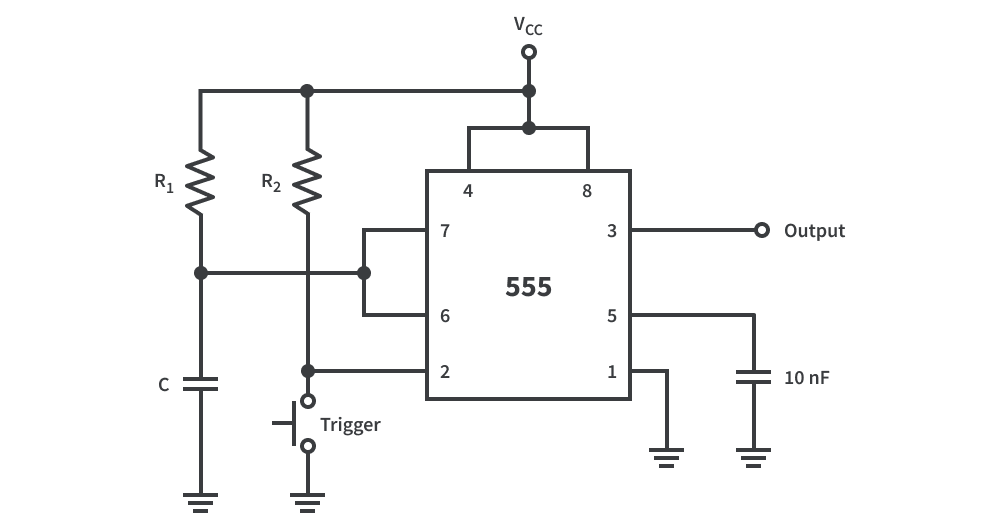
\includegraphics[width=14cm]{Pic/Pictures/555-timer-monostable-operation-schematic-diagram.png}
    \caption{NE555 Monostable mode.}
    \label{fig:enter-label}
\end{figure}

\newpage
\subsubsection{Astable Mode}

\begin{itemize}
    \item In astable mode, the 555 functions as an oscillator, producing a continuous square wave.
    \item The frequency and duty cycle of the output waveform are determined by external resistors (R1, R2) and capacitor (C).
\end{itemize}

\vspace{10pt}
\textbf{The frequency (f)} is given by: $f = \frac{1.44}{(R1 + 2 \times R2) \times C}$.\par
\textbf{The duty cycle (D)} is determined by the ratio: $\frac{R2}{R1 + 2 \times R2}$.\par

\vspace{10pt}
\textbf{Operation Steps:}
\begin{itemize}
    \item The external resistors R1 and R2, and the capacitor C, set the charging and discharging times.
    \item The voltage across the capacitor varies between the upper (2/3 Vcc) and lower (1/3 Vcc) thresholds.
    \item The 555 continuously oscillates between these thresholds.
\end{itemize}

\vspace{10pt}
\textbf{Applications:} Astable mode is commonly used for generating clock pulses, tone generation, or LED flashers.

\begin{figure}[h]
    \centering
    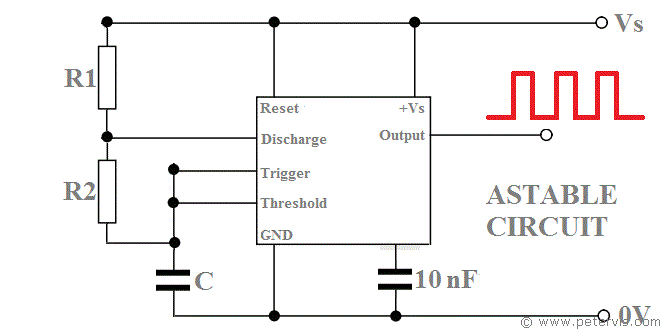
\includegraphics[width=10cm]{Pic/Pictures/555-timer-astable-circuit.png}
    \caption{NE555 Astable mode.}
    \label{fig:enter-label}
\end{figure}

In this assignment, we will use the \textbf{Astable Mode} to generate the clock pulse.

\begin{figure}[h]
    \centering
    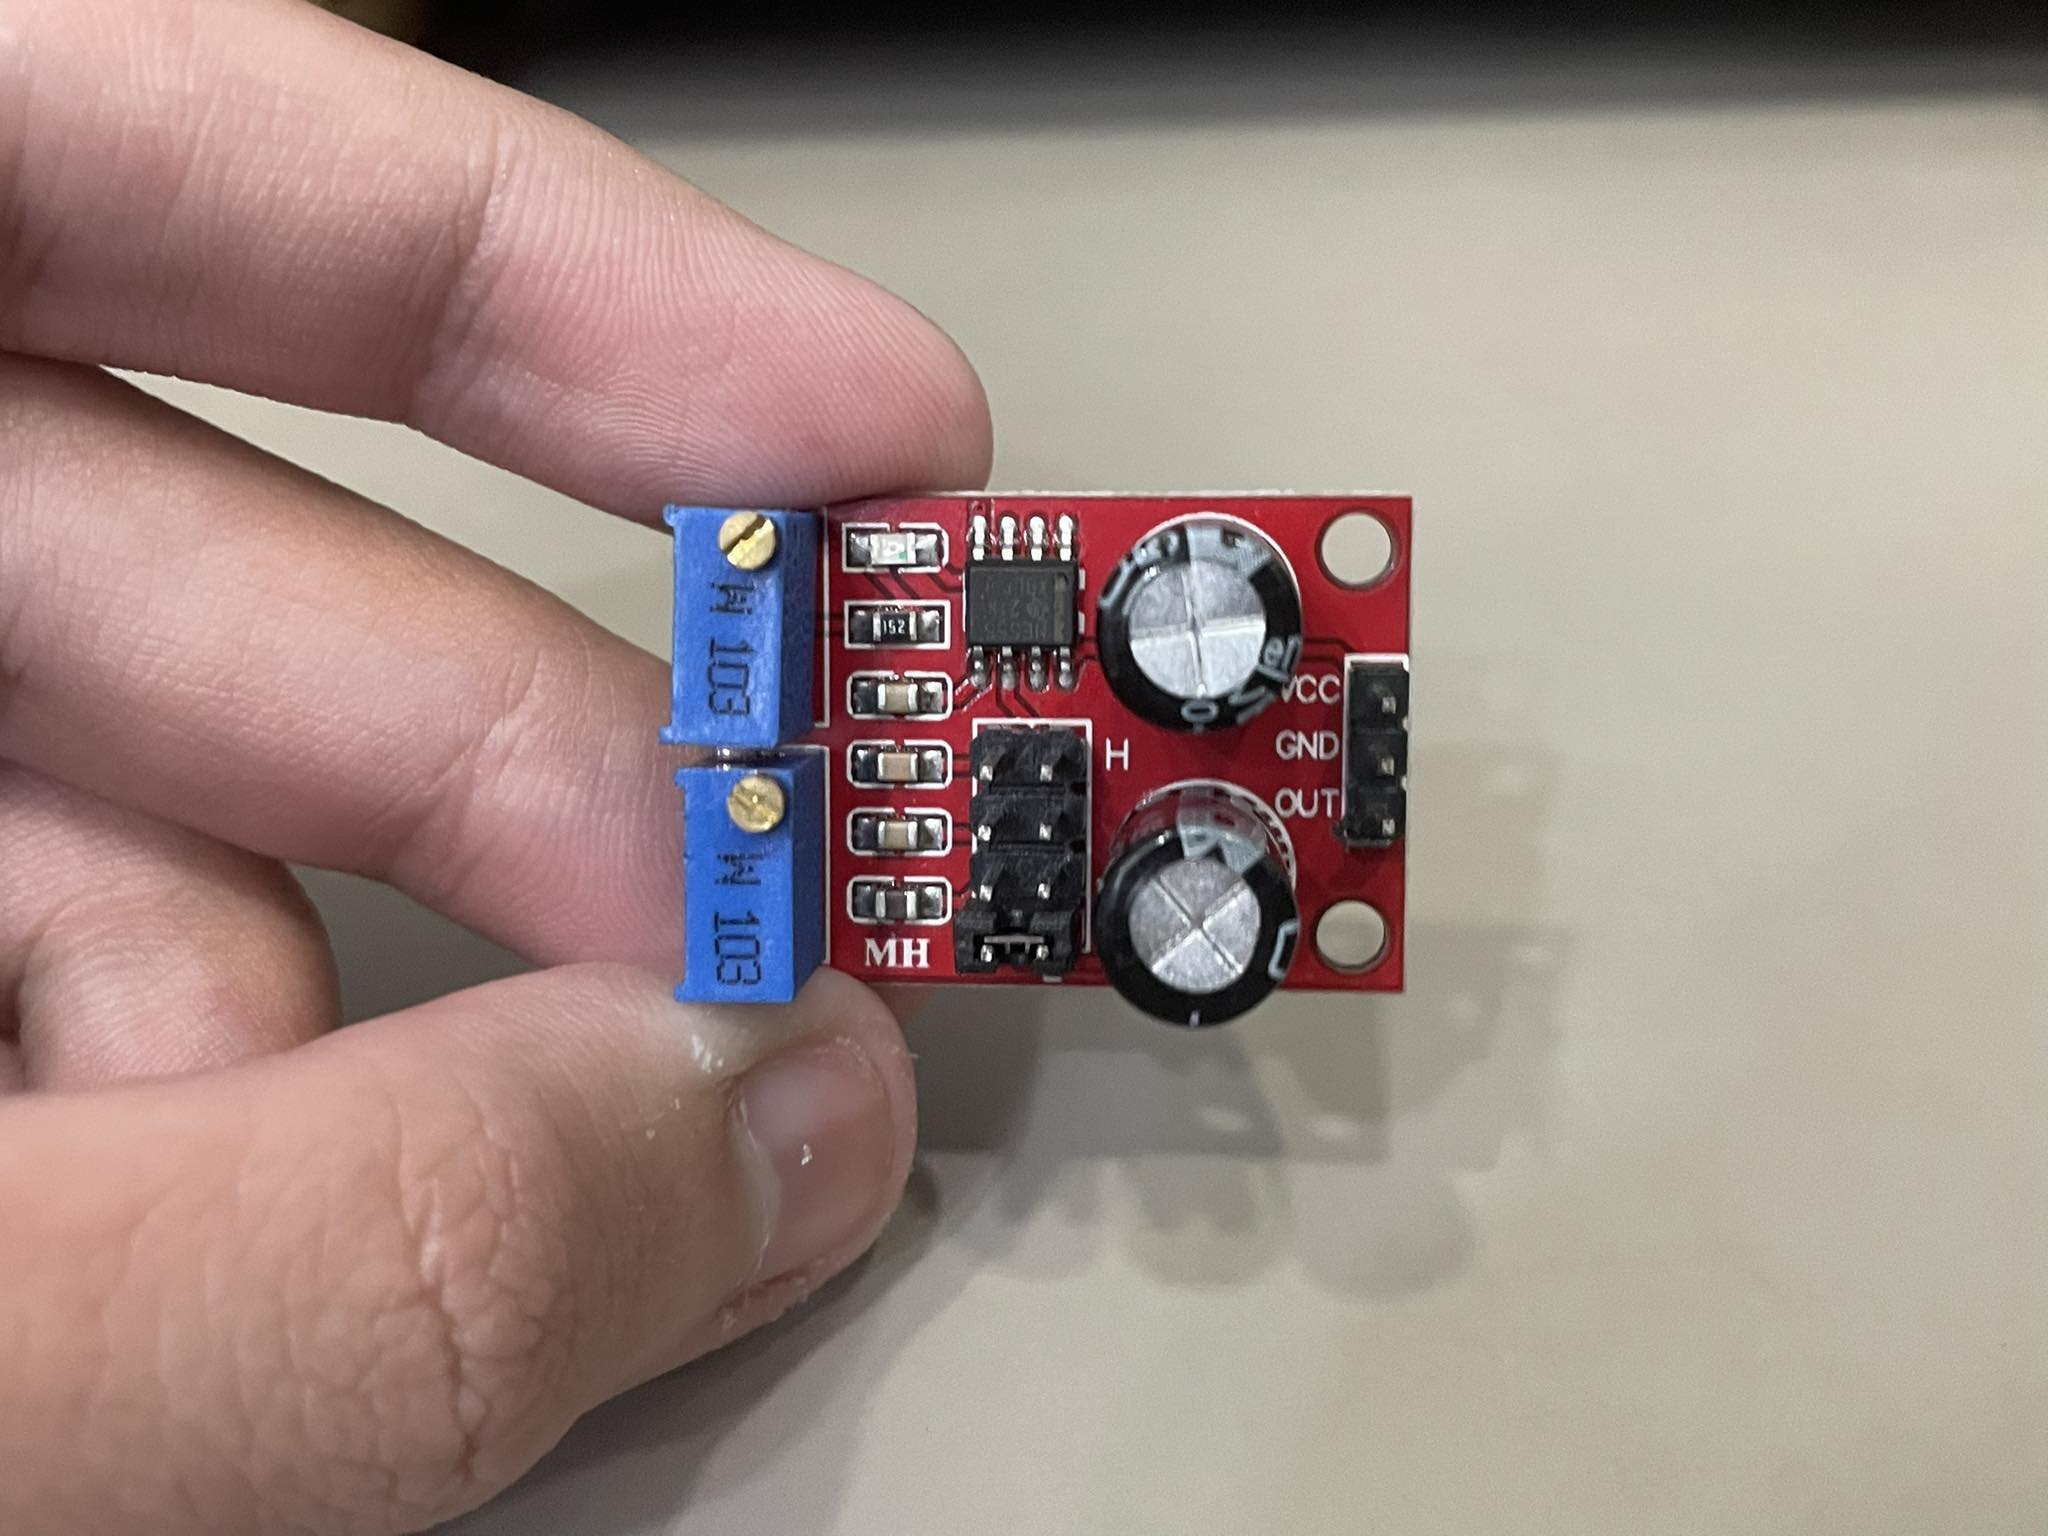
\includegraphics[width=10cm]{Pic/Pictures/NE555 real.jpg}
    \caption{NE555 Module in Real Life.}
    \label{fig:enter-label}
\end{figure}
\newpage

\subsection{How SN74LS175N Work}
The SN74LS175N is a quad D-type flip-flop IC (Integrated Circuit) from the SN74LS family. It contains four individual D-type flip-flops, each capable of storing a single bit of data.\par

\subsubsection{Basic Functionality}\par
\begin{itemize}
    \item \textbf{Single Flip-Flop:} A D-type flip-flop, or data flip-flop, stores a single bit of data (0 or 1). It has two inputs: Data (D) and Clock (CLK). The output (Q) represents the stored data.
    \item \textbf{Quad Configuration:} The SN74LS175N contains four identical D-type flip-flops (labeled A, B, C, and D). Each flip-flop operates independently of the others.
\end{itemize}

\subsubsection{Pin Configuration}
\begin{itemize}
    \item \textbf{Data Inputs (D0-D3):} These pins (4, 5, 12, and 13) are connected to the data inputs of the respective flip-flops (A, B, C, and D).
    \item \textbf{Clock Input (CLK):} Pin 9 (CLK) is the clock input shared by all four flip-flops. A rising or falling edge of the clock triggers the transfer of data to the flip-flops.
    \item \textbf{Master Reset (MR):} Pin 1 (MR) allows to asynchronously reset the internal state of the IC. When the MR input is taken low (logic 0), it forces the flip-flops or registers to a predefined state, often the reset state.
    \item \textbf{Q Outputs (Q0-Q3):} Pins 2, 7, 10, and 15 (Q0, Q1, Q2, and Q3) are the individual Q outputs of the flip-flops.
    \item \textbf{Complementary Outputs ($\overline{QO} - \overline{Q3}$):} Pins 3, 6, 11, and 14 ($\overline{Q0}$, $\overline{Q1}$, $\overline{Q2}$, and $\overline{Q3}$) provide the complementary outputs of the Q outputs.
\end{itemize}

\begin{figure}[h]
    \centering
    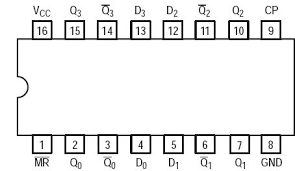
\includegraphics[width=7cm]{Pic/Pictures/175N.png}
    \caption{SN74LS175N Pins.}
    \label{fig:enter-label}
\end{figure}

\subsubsection{Operation}
\begin{itemize}
    \item \textbf{Clock Triggered Operation:} On each rising (or falling) edge of the clock (CLK), the data present at the D inputs is transferred to the Q outputs.
    \item \textbf{Independent Operation:} Each flip-flop (A, B, C, D) operates independently, allowing the IC to store four separate bits of data.
\end{itemize}

\subsubsection{Applications}
\begin{itemize}
    \item Data Storage: Used for storing binary data in digital systems.
    \item Registers: Part of digital registers and memory units in microprocessor-based systems.
    \item Clocked Circuits: Employed in clocked circuits where data needs to be synchronized with a clock signal.
    \item Sequential Logic: Forms the building block for sequential logic circuits.
\end{itemize}

The SN74LS175N provides a convenient way to implement D-type flip-flops in digital circuits, offering versatility and reliability in various applications. In this assignment, it will be used to set values to the SN74LS193N.\par

\begin{figure}[h]
    \centering
    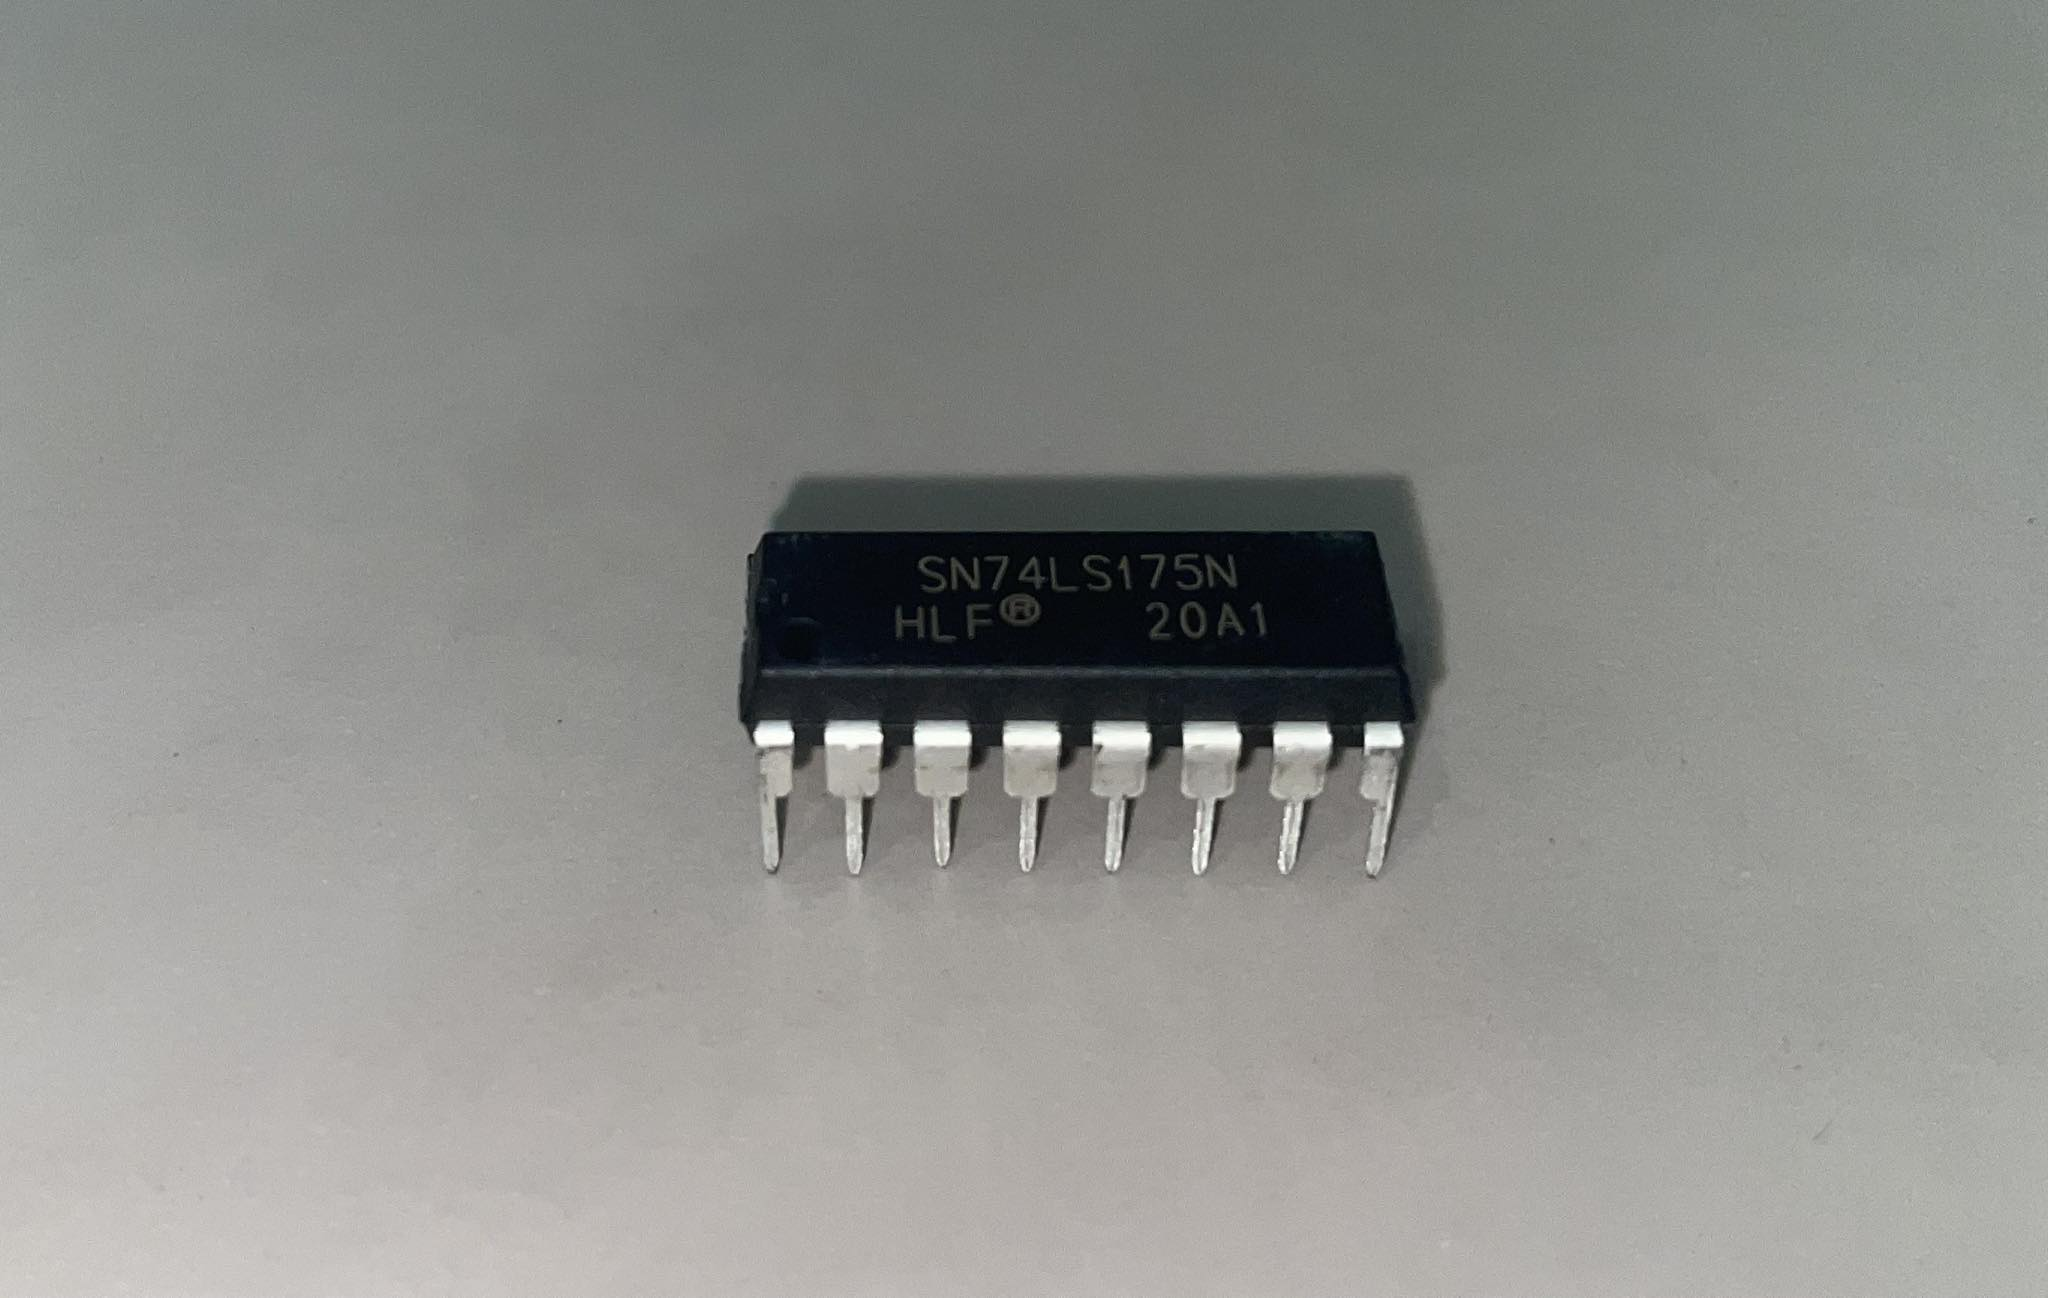
\includegraphics[width=12cm]{Pic/Pictures/175N real.jpg}
    \caption{SN74LS175N in real life.}
    \label{fig:enter-label}
\end{figure}

\newpage
\subsection{How SN74LS193N Work}
The SN74LS193N is a synchronous 4-bit binary up/down counter IC (Integrated Circuit) from the SN74LS family. It's designed to count in both upward (increment) and downward (decrement) directions.

\subsubsection{Basic Functionality}

\begin{itemize}
    \item \textbf{Binary Counter:} The SN74LS193N is a 4-bit binary counter, meaning it can count in binary from 0 to 15 ($2^4 - 1$).
    \item \textbf{Up/Down Functionality:} It can operate as an up counter (incrementing) or a down counter (decrementing), depending on the control inputs.
\end{itemize}

\subsubsection{Pin Configuration}
\begin{itemize}
    \item \textbf{Data Inputs (A, B, C, D):} Pins 15, 1, 10 and 9 (D0, D1, D2, D3) are the data inputs representing the current count value.
    \item \textbf{QA, QB, QC, QD Outputs:} Pins 3, 2, 6, and 7 (QA, QB, QC, QD) are the individual Q outputs representing the binary count.
    \item \textbf{$\mathbf{CP_{D}}$ - Clock Input (Down):} Pin 4, this is the clock input for counting down. The counter advances on the falling edge of the $CP_D$ signal. When a low-to-high transition occurs on $CP_D$, the counter decrements by one.
    \item \textbf{$\mathbf{CP_{U}}$ - Clock Input (Up):} Pin 5, this is the clock input for counting up. The counter advances on the falling edge of the $CP_U$ signal. When a low-to-high transition occurs on $CP_U$, the counter increments by one.
    \item \textbf{PL - Parallel Load Input:} Pin 11, when the input is LOW, information present on the Parallel Data inputs (D0 to D3) is loaded into the counter.
    \item \textbf{MR - Master Reset Input:} Pin 14, this is the master reset input. A HIGH signal on the Master Reset input will disable the preset gates, override both Clock inputs, and latch each Q output in the LOW state.
    \item \textbf{The Terminal Count Up (TCU) and Terminal Count Down(TCD) outputs:} Pin 12, 13 are normally HIGH. When a circuit has reached the maximum count state (15 for the LS193), the next HIGH-to-LOW transition of the Count Up Clock will cause TCU to go LOW. TCU will stay LOW until CPU goes HIGH again, thus effectively repeating the Count Up Clock, but delayed by two gate delays. Similar with the TCD.
\end{itemize}


\begin{figure}[h]
    \centering
    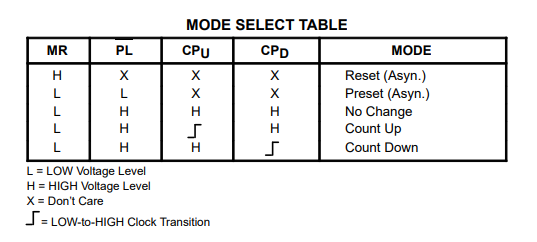
\includegraphics[width=7cm]{Pic/Pictures/193N table.png}
    \caption{Mode select table.}
    \label{fig:enter-label}
\end{figure}

\begin{figure}[h]
    \centering
    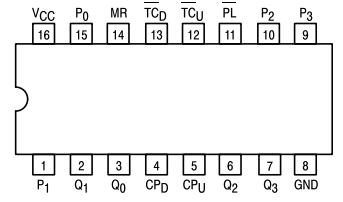
\includegraphics[width=7cm]{Pic/Pictures/193N.png}
    \caption{SN74LS193N Pins.}
    \label{fig:enter-label}
\end{figure}

\newpage

\subsubsection{Operation}
\begin{itemize}
    \item \textbf{Upward Counting:} The counter increments (counts up) on each rising edge of the clock.
    \item \textbf{Downward Counting:} The counter decrements (counts down) on each rising edge of the clock.
    \item \textbf{Loading Data:} When PL is LOW, the counter loads data from A, B, C, D inputs into the count register on the next clock edge.
\end{itemize}




\subsubsection{Applications}
\begin{itemize}
    \item Digital Counting: Used in digital systems for counting events, pulses, or cycles.
    \item Sequential Logic: Integral part of sequential logic circuits requiring counting capabilities.
    \item Frequency Division: Employed in frequency dividers where the output frequency is a fraction of the input frequency.
    \item Cascade Counting: Cascaded with other counters for extended counting ranges.
\end{itemize}

The SN74LS193N is a versatile counter IC widely used in digital circuits for various counting applications, providing a convenient solution for binary counting tasks. In this assignment, it will use the data that was sent by the SN74LS175N in the previous section.\par

\begin{figure}[h]
    \centering
    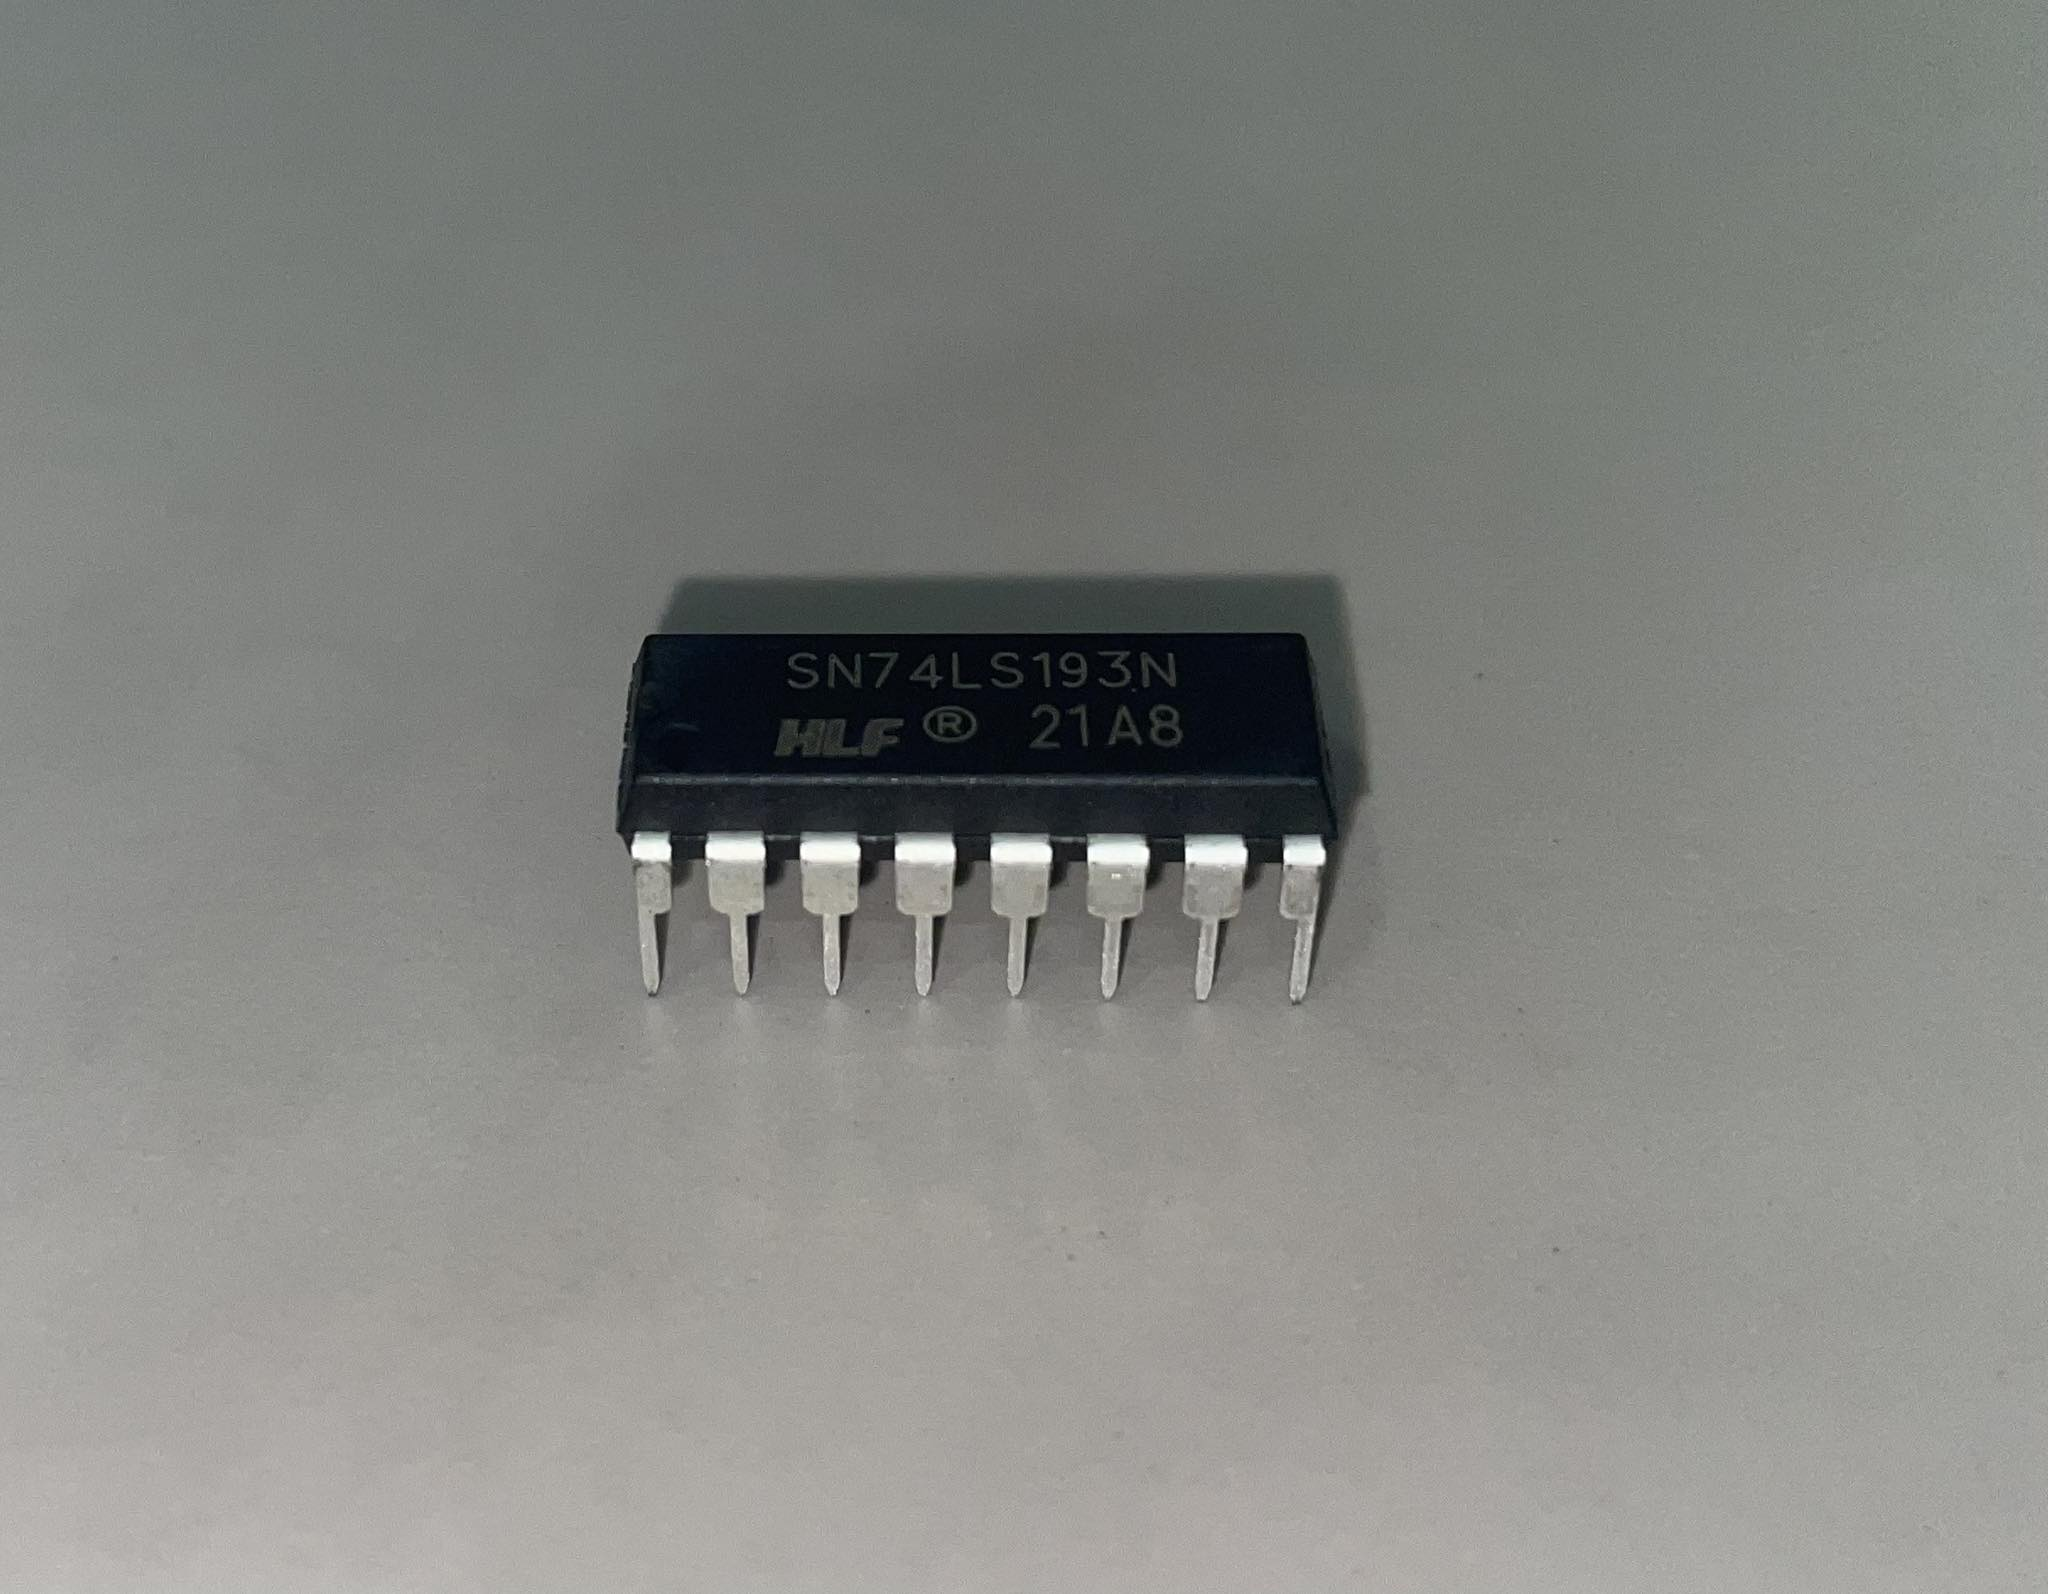
\includegraphics[width=8cm]{Pic/Pictures/193N real.jpg}
    \caption{SN74LS193N in Real Life.}
    \label{fig:enter-label}
\end{figure}



\newpage

\subsection{How CD4511BE Work}
The CD4511BE is a BCD (Binary-Coded Decimal) to 7-segment latch/decoder/driver IC. 

\subsubsection{Basic Functionality}
It is commonly used in digital display applications to convert a 4-bit BCD input into the corresponding 7-segment display outputs.\par

\subsubsection{Pin Configuration}
\begin{itemize}
    \item \textbf{Data Inputs (A, B, C, D)}: Pins 7, 1, 2, 6 are accordingly data inputs that accept a 4-bit binary-coded decimal (BCD) input (0 to 9 in binary) to represent a decimal digit.
    \item \textbf{The 7-segment outputs (a, b, c, d, e, f, g)}: Pins 13, 12, 11, 10, 9, 15, and 14, outputs for driving a 7-segment display.
    \item \textbf{The Lamp Test ($\overline{\textbf{LT}}$)}: Pin 3, this input, when low, enables the lamp test mode, lighting all LEDs.
    \item \textbf{The Blanking ($\overline{\textbf{BL}}$)}: Pin 4, when this input is low, all LEDs are turned off.
    \item \textbf{The Latch Enable or Strobe input (LE/$\overline{\textbf{STB}}$)}: Pin 5, when this input is high, the BCD input data is latched.
\end{itemize}

\begin{figure}[h]
    \centering
    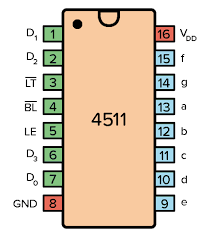
\includegraphics[width=3cm]{Pic/Pictures/4511 Pins.png}
    \caption{CD4511BE Pins.}
    \label{fig:enter-label}
\end{figure}

\subsubsection{Applications}
\begin{itemize}
    \item Digital Displays: Used in digital displays for applications like digital clocks, calculators, etc.
    \item Counters and Timers: Utilized in counting and timing circuits for displaying numerical values.
    \item Instrumentation: Integrated into various digital instrumentation systems.
    \item Cascading Multiple ICs: The BI (Blanking Input)3 pins allow multiple CD4511BE ICs to be cascaded for applications that require extended BCD counting or more digits in the display.
\end{itemize}


The CD4511BE simplifies the process of interfacing a BCD input with a 7-segment display, making it a convenient choice for numeric display applications. Proper control of latch and blanking signals is crucial for accurate and glitch-free display operation.

\begin{figure}[h]
    \centering
    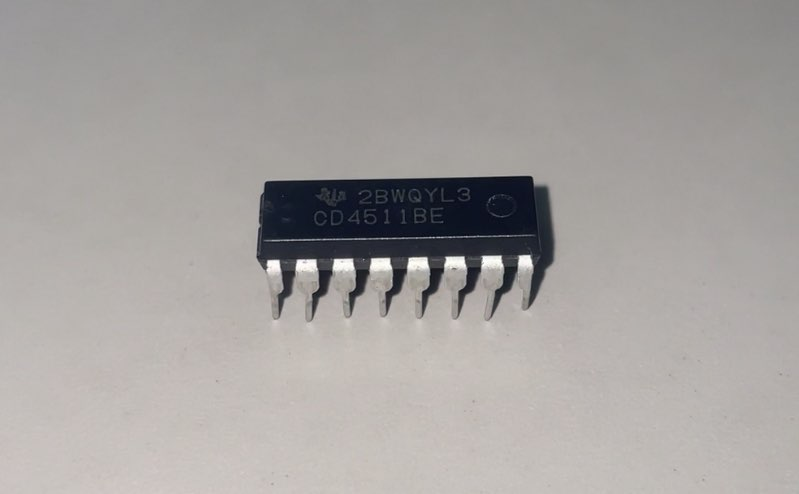
\includegraphics[width=10cm]{Pic/Pictures/4511 real.jpg}
    \caption{CD4511BE in Real Life.}
    \label{fig:enter-label}
\end{figure}
\newpage

\subsection{How CD4017BE Work}
The CD4017BE is a decade counter/divider IC that is commonly used in electronic circuits for sequential counting applications. It's a member of the CD4000 series of integrated circuits (ICs). Let's explore its basic functionality, pin configuration, operations, and applications:

\subsubsection{Basic Functionality}
The CD4017BE is commonly used in electronic circuits where sequential counting is required, such as LED chasers, digital clocks, timers, etc...

\subsubsection{Pin Configuration}
\begin{itemize}
    \item \textbf{Output pins Q0 to Q9:} Pin 1, 2, 3, 4, 5, 6, 7, 9, 10, 11. These pins are the output dedicate Q0 to Q9. Note that these pins are not in order direction with the order from Q0 to Q9.
    \item \textbf{Carry Out ($\overline{CO}$): }Pin 12, 
    \item \textbf{Clock Enable ($\overline{EN}$): }Pin 13,
    \item \textbf{Clock (CLK): }Pin 14,
    \item \textbf{Master Reset (MR): }Pin 15,
\end{itemize}

\begin{figure}[h]
    \centering
    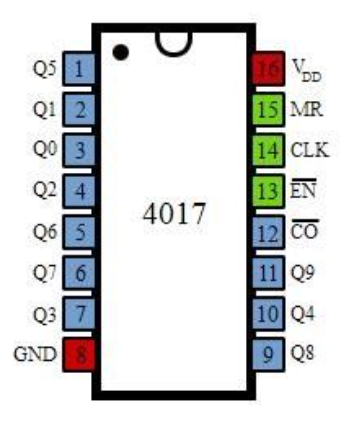
\includegraphics[width=3cm]{Pic/Pictures/4017 pins.png}
    \caption{CD4017BE Pins.}
    \label{fig:enter-label}
\end{figure}

\subsubsection{Operation}
\begin{itemize}
    \item \textbf{Clocking:} The CD4017BE counts on the rising edge of the clock signal applied to the Clock (CLK) input.
    \item \textbf{Decoding Outputs:} The Q0 to Q9 outputs represent the decimal values 0 to 9, and they go HIGH sequentially as the counter advances.
    \item \textbf{Reset Operation:} The counter can be reset to 0 by bringing the Reset (RESET) input LOW.
\end{itemize}


\subsubsection{Applications}
\begin{itemize}
    \item Sequential LED Chasers: Used in LED chaser circuits where LEDs light up sequentially.
    \item Decade Counters: Ideal for applications requiring a decade counter, such as timers and frequency dividers.
    \item Digital Dice: Employed in electronic dice circuits where the numbers on the dice are sequentially displayed.
    \item Frequency Dividers: Used in frequency divider circuits to divide the input frequency by 10.
    \item Automated Lighting Systems: Integrated into lighting control circuits for sequential lighting patterns.
\end{itemize}

The CD4017BE is a versatile and widely used IC in digital electronics, providing a straightforward solution for sequential counting applications. Its ease of use and versatility make it suitable for various hobbyist and educational projects.

\begin{figure}[h]
    \centering
    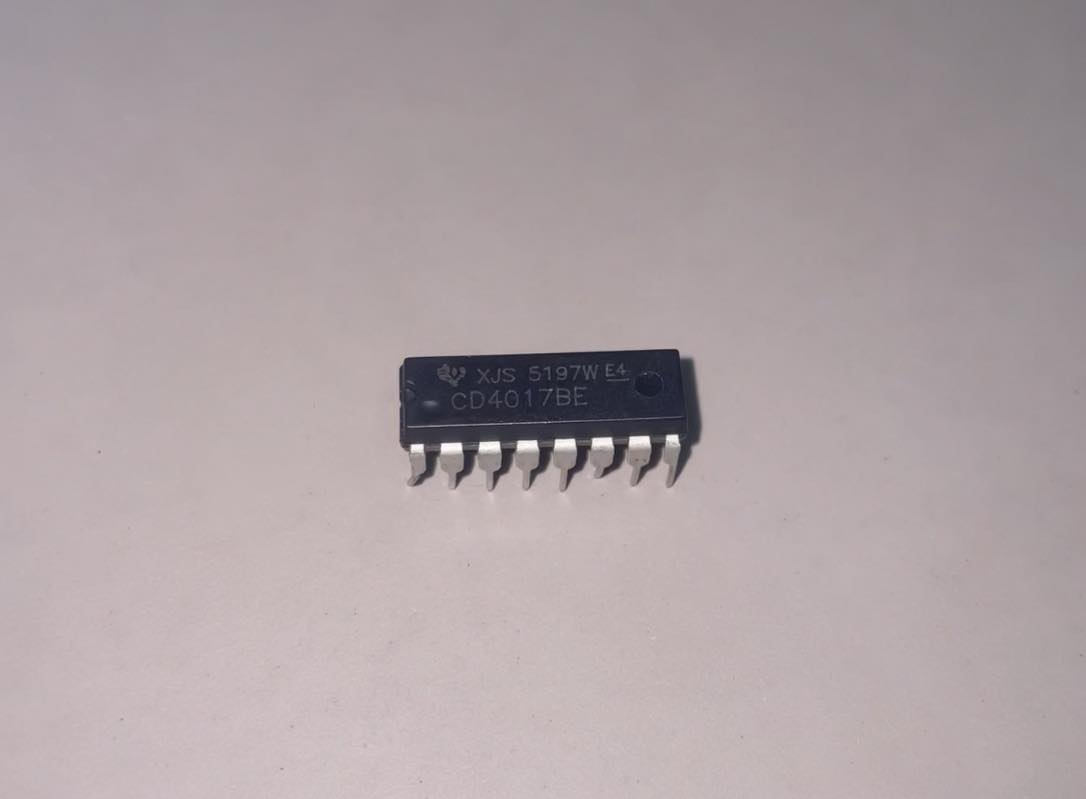
\includegraphics[width=10cm]{Pic/Pictures/4017 real.jpg}
    \caption{CD4017BE in Real Life.}
    \label{fig:enter-label}
\end{figure}
\newpage


\section{Implementation}
\subsection{Ideas to solve the problem}
\subsubsection{Simulate NE555 Module}
Creating the NE555 module is a fundamental step that involves generating a stable clock signal. Using the theory on the above, we will have the following module in proteus:\par
\begin{figure}[h]
    \centering
    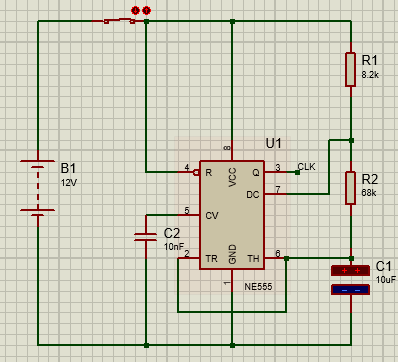
\includegraphics[width=10cm]{Pic/Proteus/NE555_Module_Proteus.png}
    \caption{NE555 with Astable Mode.}
    \label{fig:enter-label}
\end{figure}

\subsubsection{Implement signals}
In the upcoming phase of the project, we aim to incorporate two operational modes: \textbf{Automatic} and \textbf{Manual}. The Automatic mode signifies the regular operation based on predefined time durations. Conversely, the Manual mode comes into play in scenarios such as traffic congestion, allowing manual intervention by the police to modify the LED signals and avoid traffic jams. We will use a switch so that we can change each mode easily.\par

\begin{figure}[h]
    \centering
    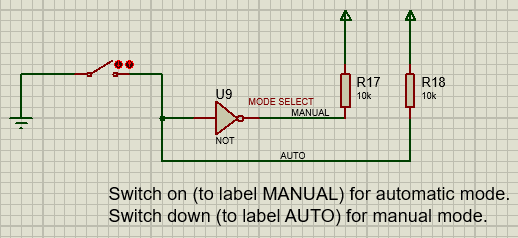
\includegraphics[width=10cm]{Pic/Proteus/Mode Selection.png}
    \caption{Mode Selection.}
    \label{fig:enter-label}
\end{figure}
\newpage

The CD4017BE is a decade counter/divider IC (integrated circuit) that is commonly used in electronic circuits. It has 10 output pins (Q0 through Q9) that sequentially turn high in response to clock pulses. The CD4017BE advances its count on each clock pulse, but it's important to note that it starts counting from a reset state when power is applied.

To prevent the first clock pulse from affecting the count, it is often necessary to include a reset circuit or a mechanism to ensure that the counter begins counting from a known state. If you allow the first clock pulse to trigger the counter without resetting it, the initial state of the counter might be unpredictable.

In our project, when operating in automatic mode, it is necessary to verify whether any outputs of the SN74LS175N are set. If none are set, the clock of the CD4017BE will be deactivated; otherwise, it will be activated as soon as active output is detected from the SN74LS175N.\par

\begin{figure}[h]
    \centering
    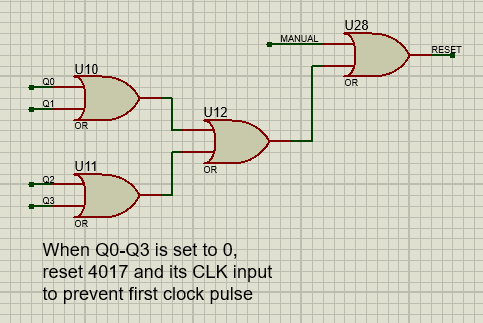
\includegraphics[width=10cm]{Pic/Proteus/Reset signal.png}
    \caption{Reset signal.}
    \label{fig:enter-label}
\end{figure}

\subsubsection{Implement First-road Traffic}
Configuring the duration of the LEDs based on their colors is a pivotal aspect of this assignment. Our team aims to achieve this by employing D Flip-Flops. The sequence is designed to transition from an initial state of \textbf{xxxx} to \textbf{1000} (representing the number 8) with the first clock pulse. Subsequently, upon the next clock pulse, the sequence shifts from \textbf{1000} to \textbf{0101} (number 5). This progression continues, with each subsequent clock pulse leading to transitions from \textbf{0101} to \textbf{0011} (number 3) and eventually returning from \textbf{0011} to \textbf{1000} (number 8). We can achieve this by using the K-map method. Here is the transition table:\par

\begin{figure}[h]
    \centering
    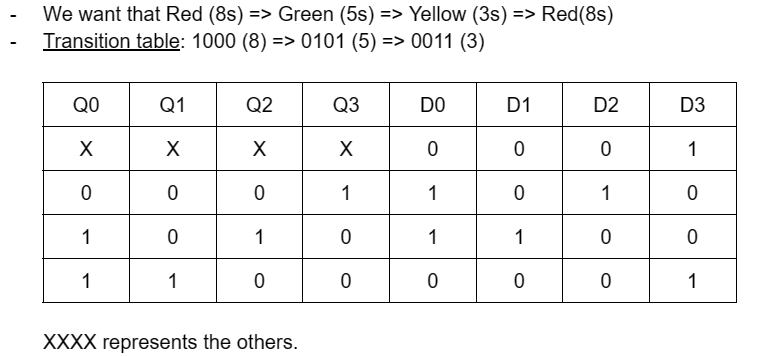
\includegraphics[width=10cm]{Pic/Proteus/transition table.png}
    \caption{Transition Table.}
    \label{fig:enter-label}
\end{figure}
\newpage
Then, we will have the truth table for D0 as follow:\par

\begin{figure}[h]
    \centering
    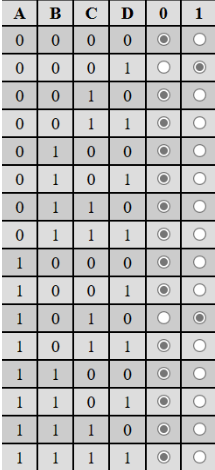
\includegraphics[width=3cm]{Pic/Proteus/Truth table D0.png}
    \caption{Truth table for D0.}
    \label{fig:enter-label}
\end{figure}

After having the truth table of D0, we will use the K-map method to solve it. After all, we will receive the equation of D0 as follow:\par
\begin{center}
    $D_0 = \overline{Q_0}.\overline{Q1}.\overline{Q2}.Q3 + Q0.\overline{Q1}.Q2.\overline{Q3}$
\end{center}

Doing the same thing with D1, D2 and D3. In summary, we will receive four specific equation so that the transition will be as we expected before. Here are the equations:\par
\vspace{10pt}
$D_0 = \overline{Q_0}.\overline{Q1}.\overline{Q2}.Q3 + Q0.\overline{Q1}.Q2.\overline{Q3}$\par
$D_1 = Q0.\overline{Q1}.Q2.\overline{Q3}$\par
$D_2 = \overline{Q_0}.\overline{Q1}.\overline{Q2}.Q3$\par
$D_3 = Q1 + \overline{Q0}.\overline{Q3} + Q2.Q3 + Q0.\overline{Q2}$
\vspace{10pt}

Now, just implement the above equations in Proteus and see the result.\par
\begin{figure}[h]
    \centering
    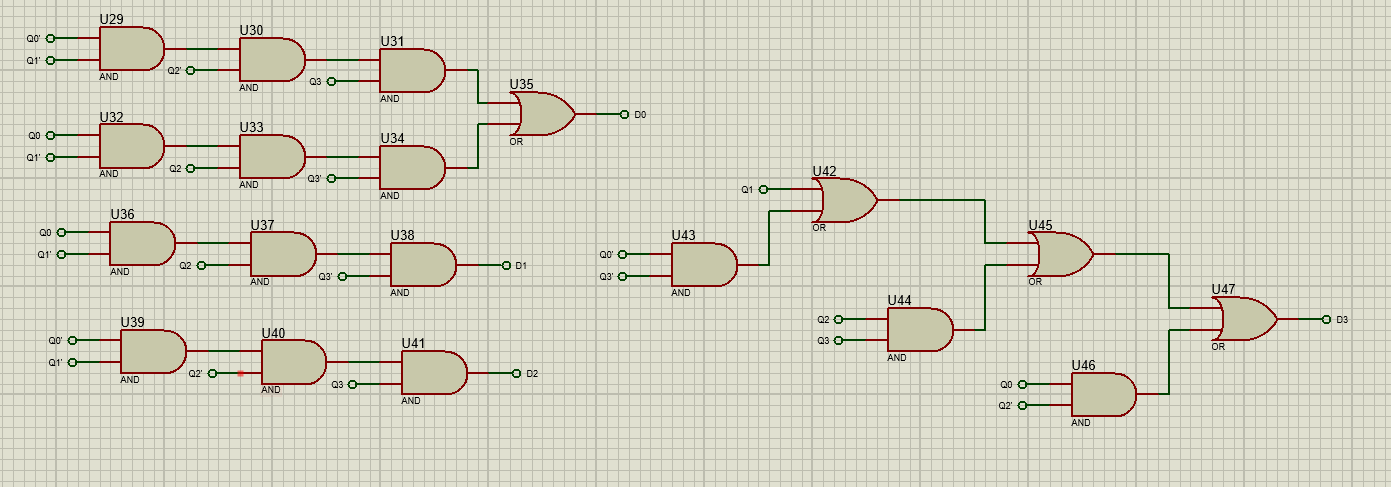
\includegraphics[width=10cm]{Pic/Proteus/175N_Proteus_0.png}
    \caption{Setting D0 to D3 to meet conditions.}
    \label{fig:enter-label}
\end{figure}
\newpage

Using three designated ICs as outlined in the preceding section, namely \textbf{SN74LS175N}, \textbf{SN74LS193N}, and \textbf{CD4511BE}, we have the capability to emulate a 7-segment signal. This signal initiates from 8, undergoes a countdown, transitions to 5, repeats the countdown, further changes to 3, continues the countdown, and cyclically returns to 8.\par

\begin{figure}[h]
    \centering
    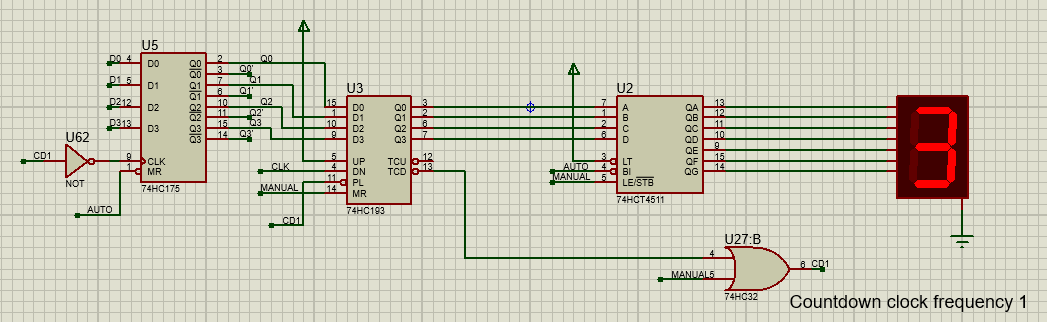
\includegraphics[width=10cm]{Pic/Proteus/175N_Proteus_1.png}
    \caption{Implement the 7-segment led for the first road.}
    \label{fig:enter-label}
\end{figure}

After finishing developing the 7-segment signal for the first road, we will then go to the next step is to configure the traffic light. Using the IC CD4017 to leverage its Sequential LED Chasers application. Here is how we simulate it in Proteus:\par
\begin{figure}[h]
    \centering
    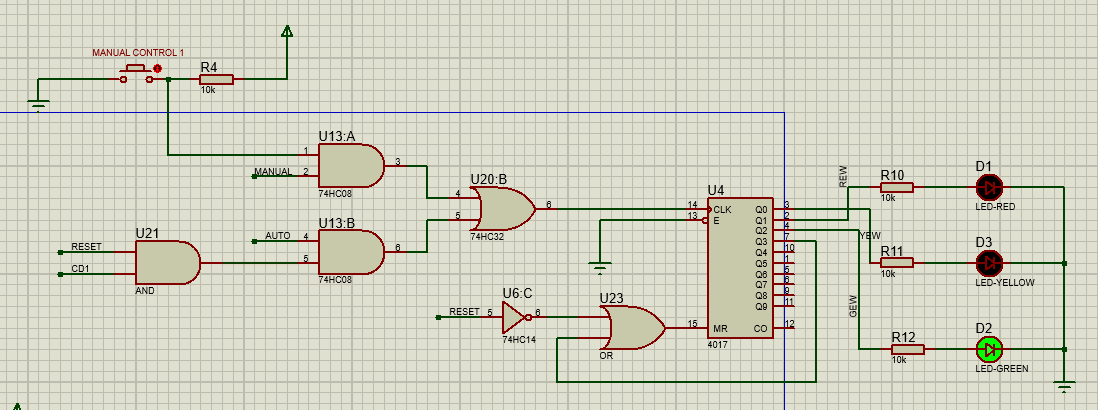
\includegraphics[width=10cm]{Pic/Proteus/4017_Proteus_0.png}
    \caption{Implement the first road.}
    \label{fig:enter-label}
\end{figure}

In the \textbf{Automatic Mode}, the triggering of the CLK signal in CD4017BE is contingent upon receiving the signal from CD1. CD1 is activated solely when the SN74LS193N reaches a countdown of 0 in our simulation. Another scenario in this mode involves the CLK being activated upon receiving a Reset signal, specifically designated to manage the first clock pulse signal from NE555.\par
In the \textbf{Manual Mode}, the CLK signal will be triggered only when we press the button. It means that every time we press, we can change the light signal of the road. That is why it is called "Manual".\par

In conclusion, the outcome will unfold as follows: The red light will persist for 8 seconds, transitioning to green light for 5 seconds, and concluding with 3 seconds of yellow light. In the Manual mode, each press of the button will bring about a change in the light signal. Now we will changing to the other road.\par

\newpage
\subsubsection{Implement Second-road Traffic}
First of all is to configure the 7-segment led signal for this road. The idea is the same with the above. However, the transition table is different because this road will start with different state frome the above. Here is the transition table for this road:\par
\begin{figure}[h]
    \centering
    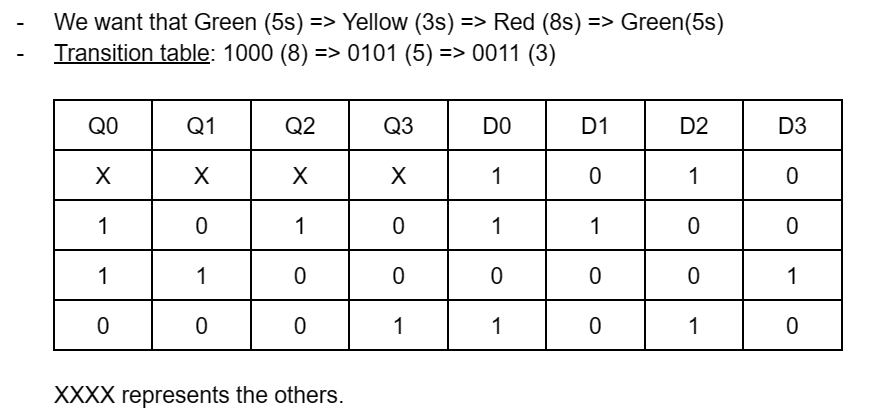
\includegraphics[width=10cm]{Pic/Proteus/transition table 2.png}
    \caption{Transition table for Second-road.}
    \label{fig:enter-label}
\end{figure}

And we also have the truth table for D0 of this road as: \par
\begin{figure}[h]
    \centering
    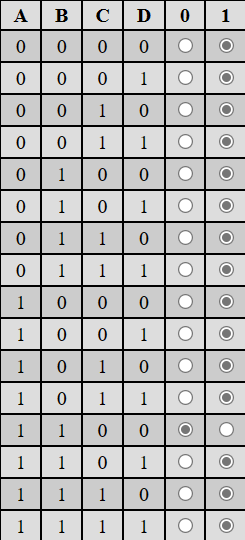
\includegraphics[width=3cm]{Pic/Proteus/Truth table D0_2.png}
    \caption{Truth table for D0 of Second-road.}
    \label{fig:enter-label}
\end{figure}

Apply the same with D1, D2, D3. Using k-map, we will have the following:\par
$D0 = \overline{Q0} + \overline{Q1} + Q2 + Q3$\par
$D1 = Q0.\overline{Q1}.Q2.\overline{Q3}$\par
$D2 = \overline{Q0} + Q3 + \overline{Q1}.\overline{Q2} + Q1.Q2$\par
$D3 = Q0.Q1.\overline{Q2}.\overline{Q3}$\par

Here is how we implement those equations in Proteus:\par
\begin{figure}[h]
    \centering
    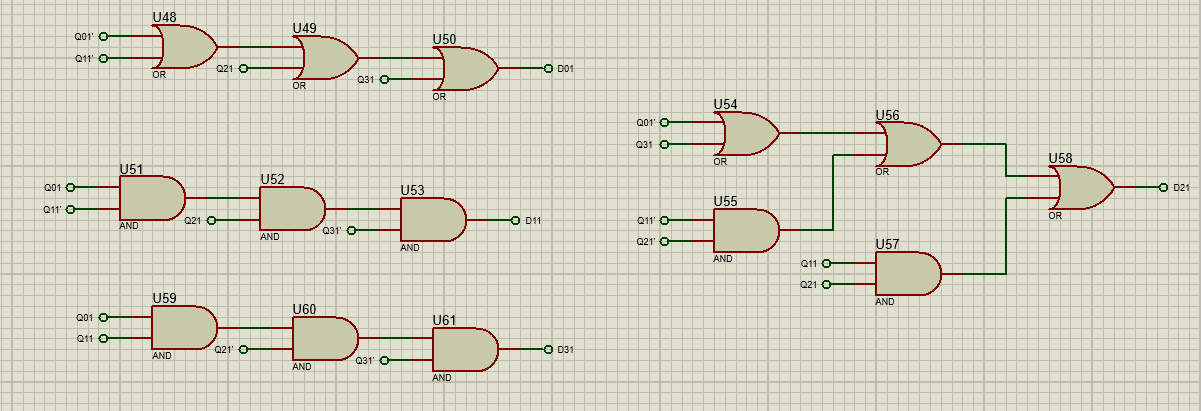
\includegraphics[width=10cm]{Pic/Proteus/175N_Proteus_2.png}
    \caption{Setting D00 to D03 to meet conditions.}
    \label{fig:enter-label}
\end{figure}


By utilizing three specific ICs, as discussed in the above section, namely SN74LS175N, SN74LS193N, and CD4511BE, we can simulate the 7-segment signal. It will initially display the number 5 and then count down. Subsequently, it will transition to 3 and count down, followed by changing to 8 and counting down. The cycle repeats, ultimately returning to the number 5.\par
\begin{figure}[h]
    \centering
    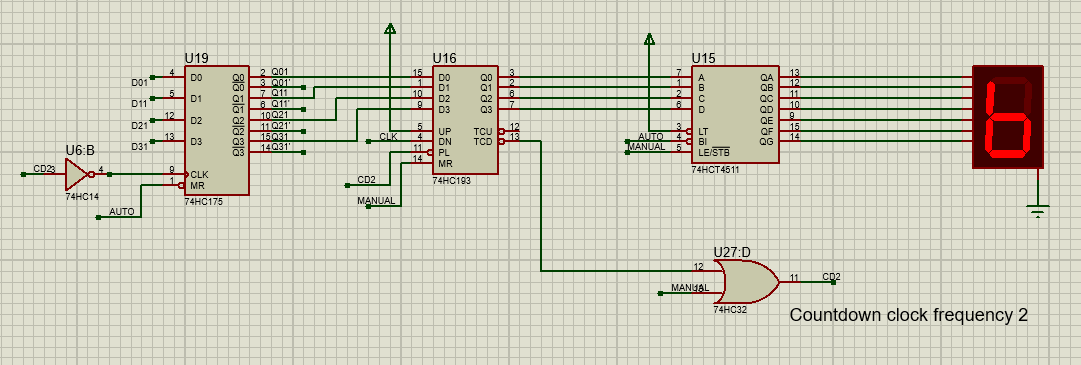
\includegraphics[width=10cm]{Pic/Proteus/175N_Proteus_3.png}
    \caption{Implement the 7-segment led for the second road.}
    \label{fig:enter-label}
\end{figure}


Proceeding to the subsequent phase involves configuring the signals for the LEDs. Since our group designated the previous road as the primary one, the light signals on this secondary road are depend on the signals from the main road. In the \textbf{Automatic Mode}, we can define the signals according to the established theory. However, in the \textbf{Manual Mode}, the signals are now reliant on those of the main road.\par
For detail, in \textbf{Manual Mode}, if the led signals in the main road is RED, this road should be GREEN and vice versa. For the YELLOW, both of the roads will have the same color.\par 

\begin{figure}[h]
    \centering
    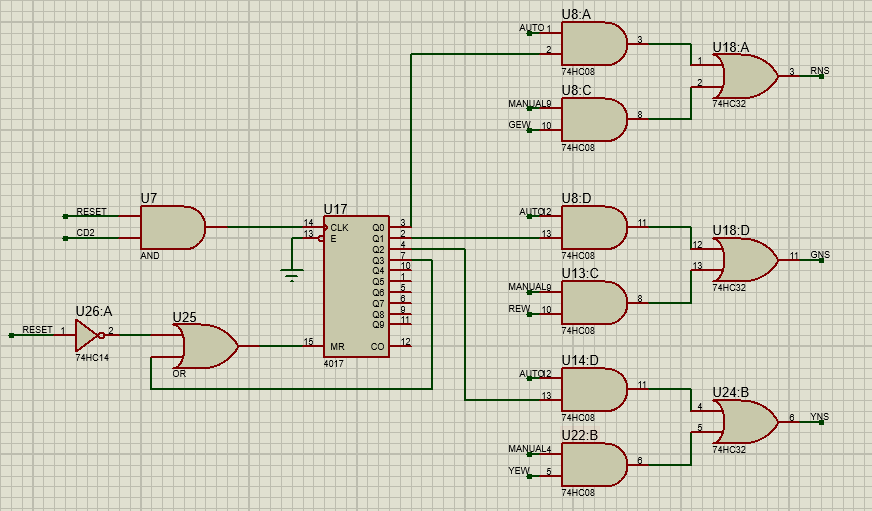
\includegraphics[width=10cm]{Pic/Proteus/4017_Proteus_1.png}
    \caption{Implement the second road.}
    \label{fig:enter-label}
\end{figure}

And that is the end of our implementation of the problem "Four-way Traffic Light". For detail output, moving to the next section.\par
\newpage

\subsection{Proteus Simulation}
First of all, we will check out our \textbf{Automatic Mode}. In this mode, there are 4 states namely: RED-GREEN, RED-YELLOW, GREEN-RED, YELLOW-RED. And here are the outputs of our implementation in Automatic Mode.\par

\begin{figure}[h]
    \centering
    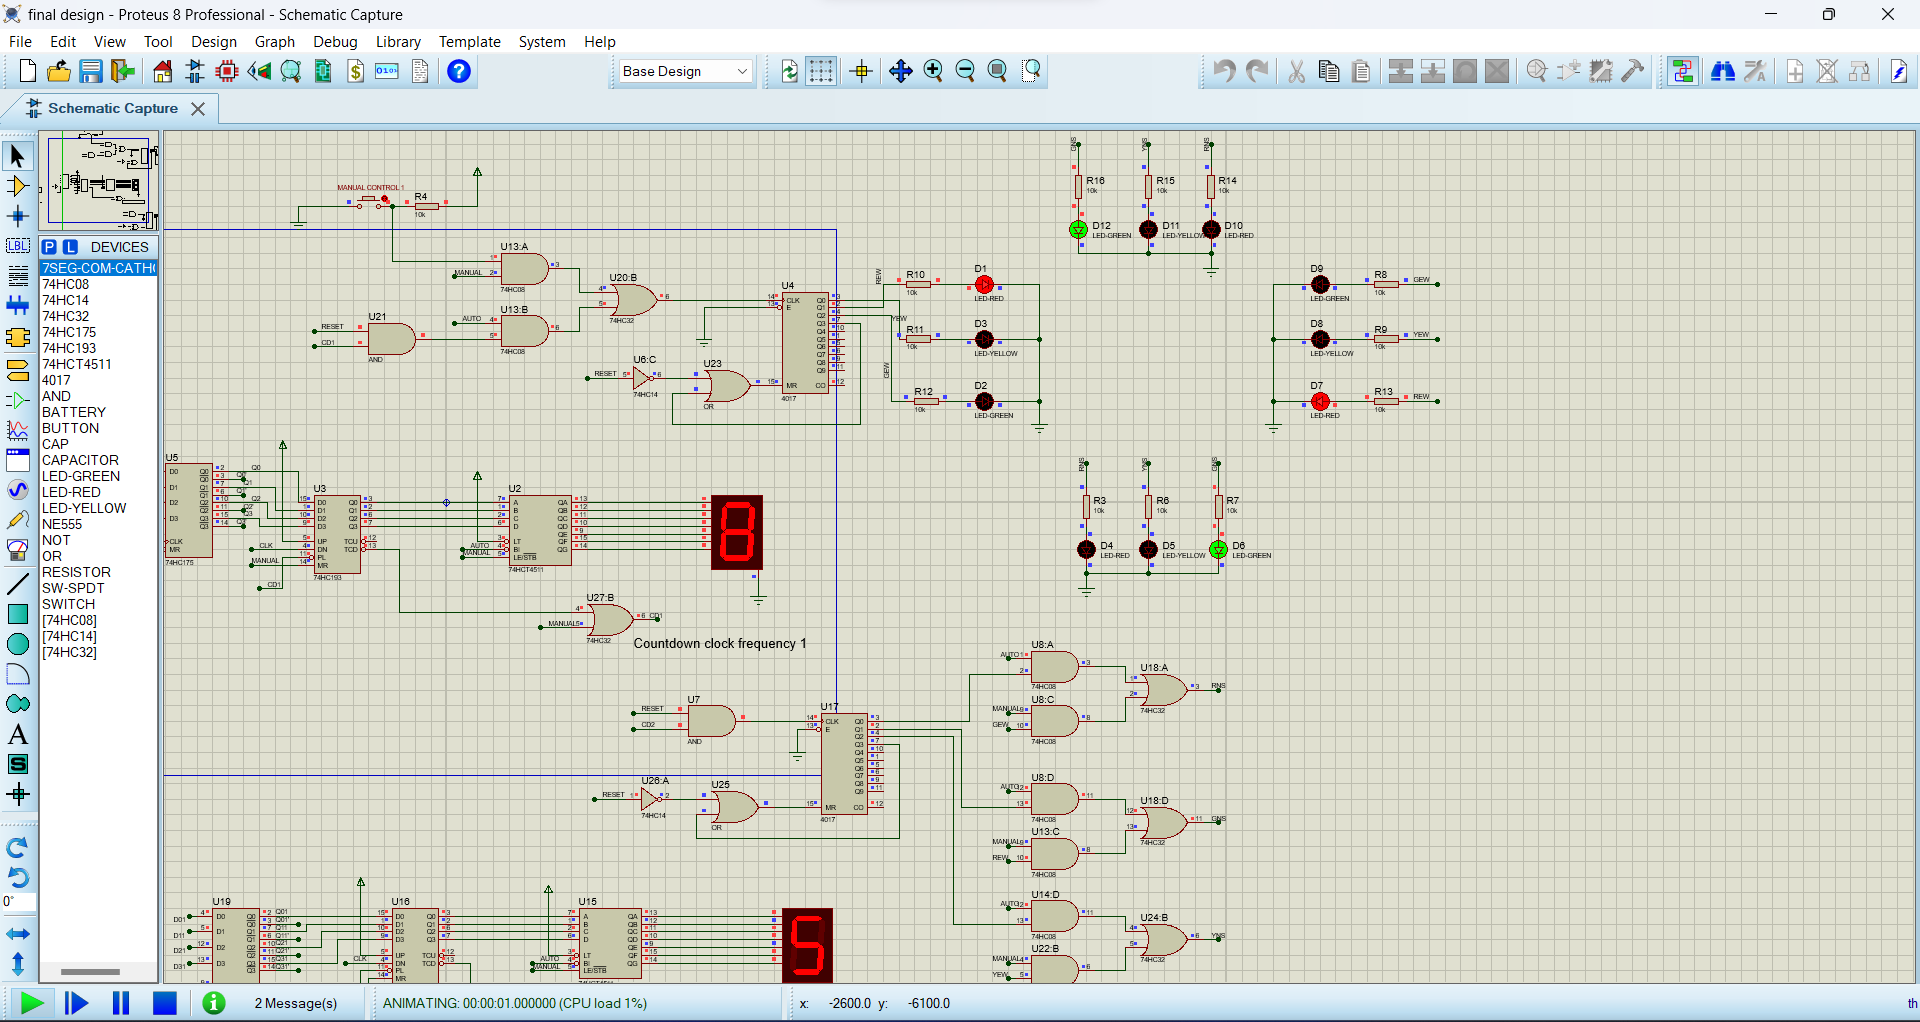
\includegraphics[width=14cm]{Pic/Proteus/Automatic_0.png}
    \caption{State RED-GREEN.}
    \label{fig:enter-label}
\end{figure}

\begin{figure}[h]
    \centering
    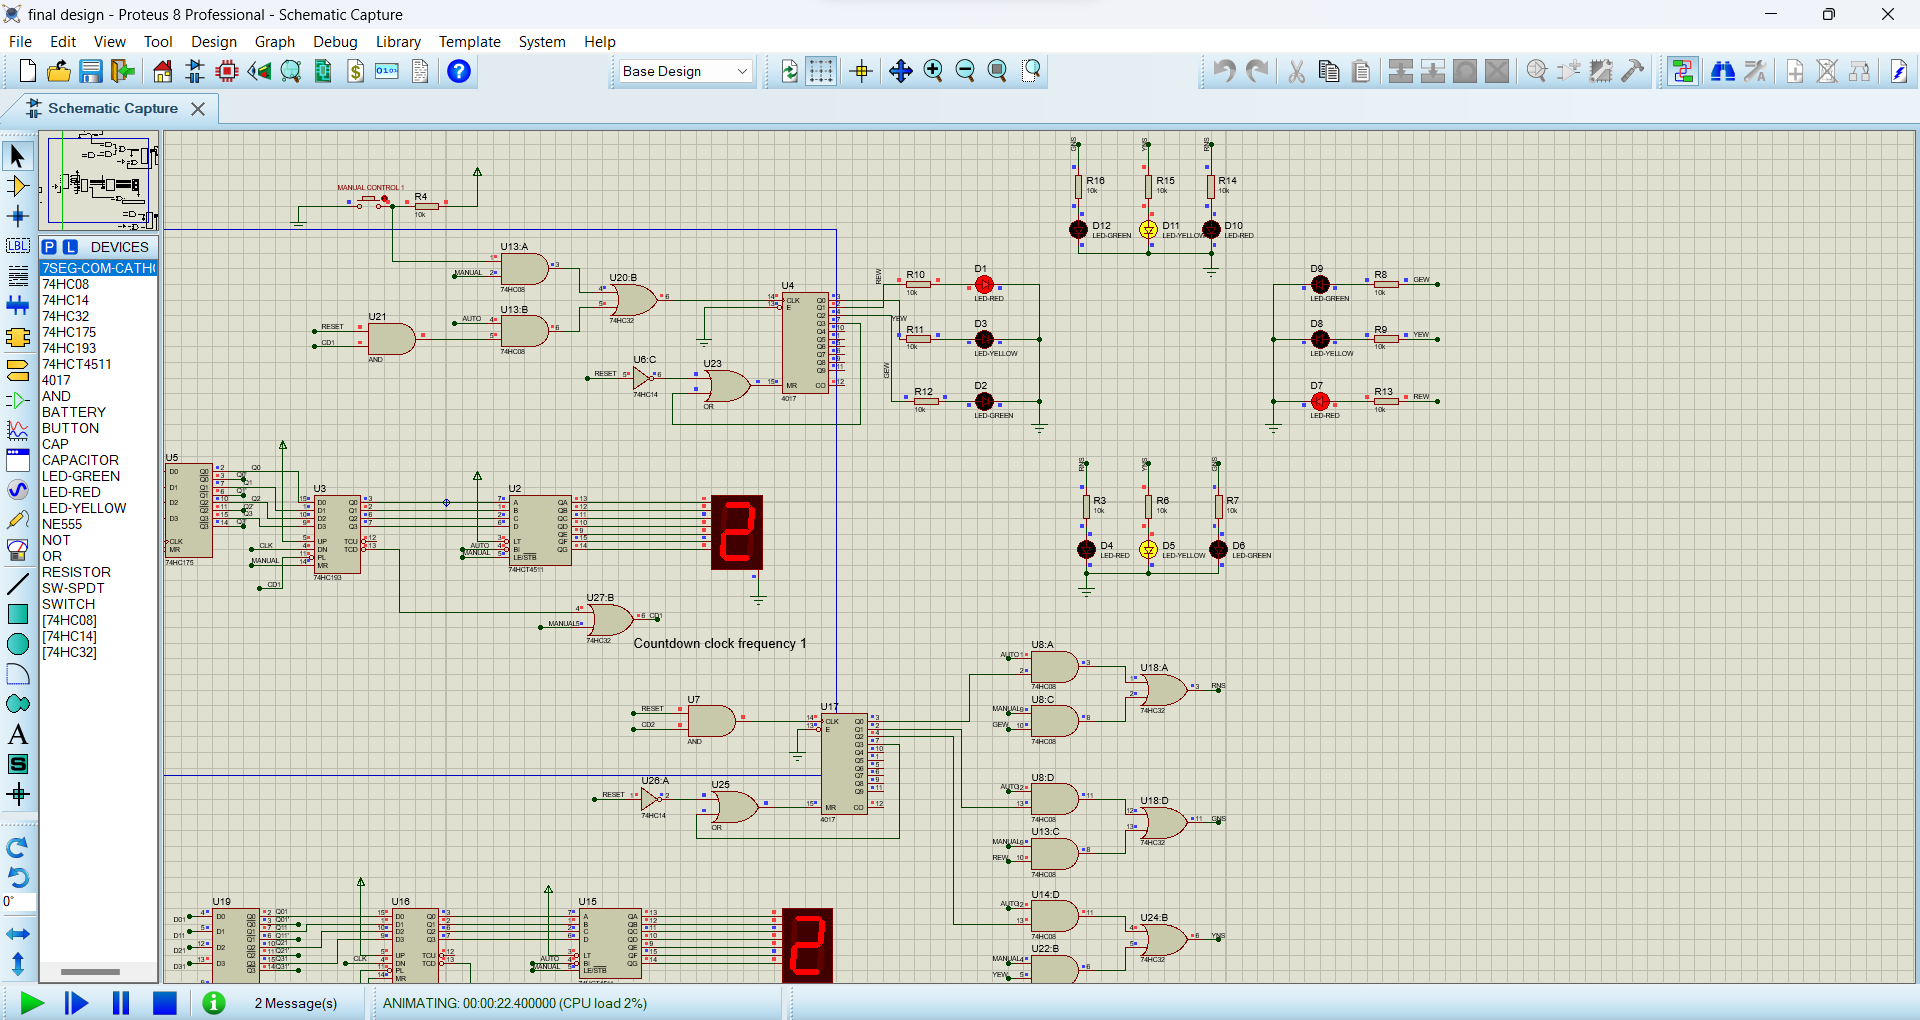
\includegraphics[width=14cm]{Pic/Proteus/Automatic_1.png}
    \caption{State RED-YELLOW.}
    \label{fig:enter-label}
\end{figure}

\newpage

\begin{figure}[h]
    \centering
    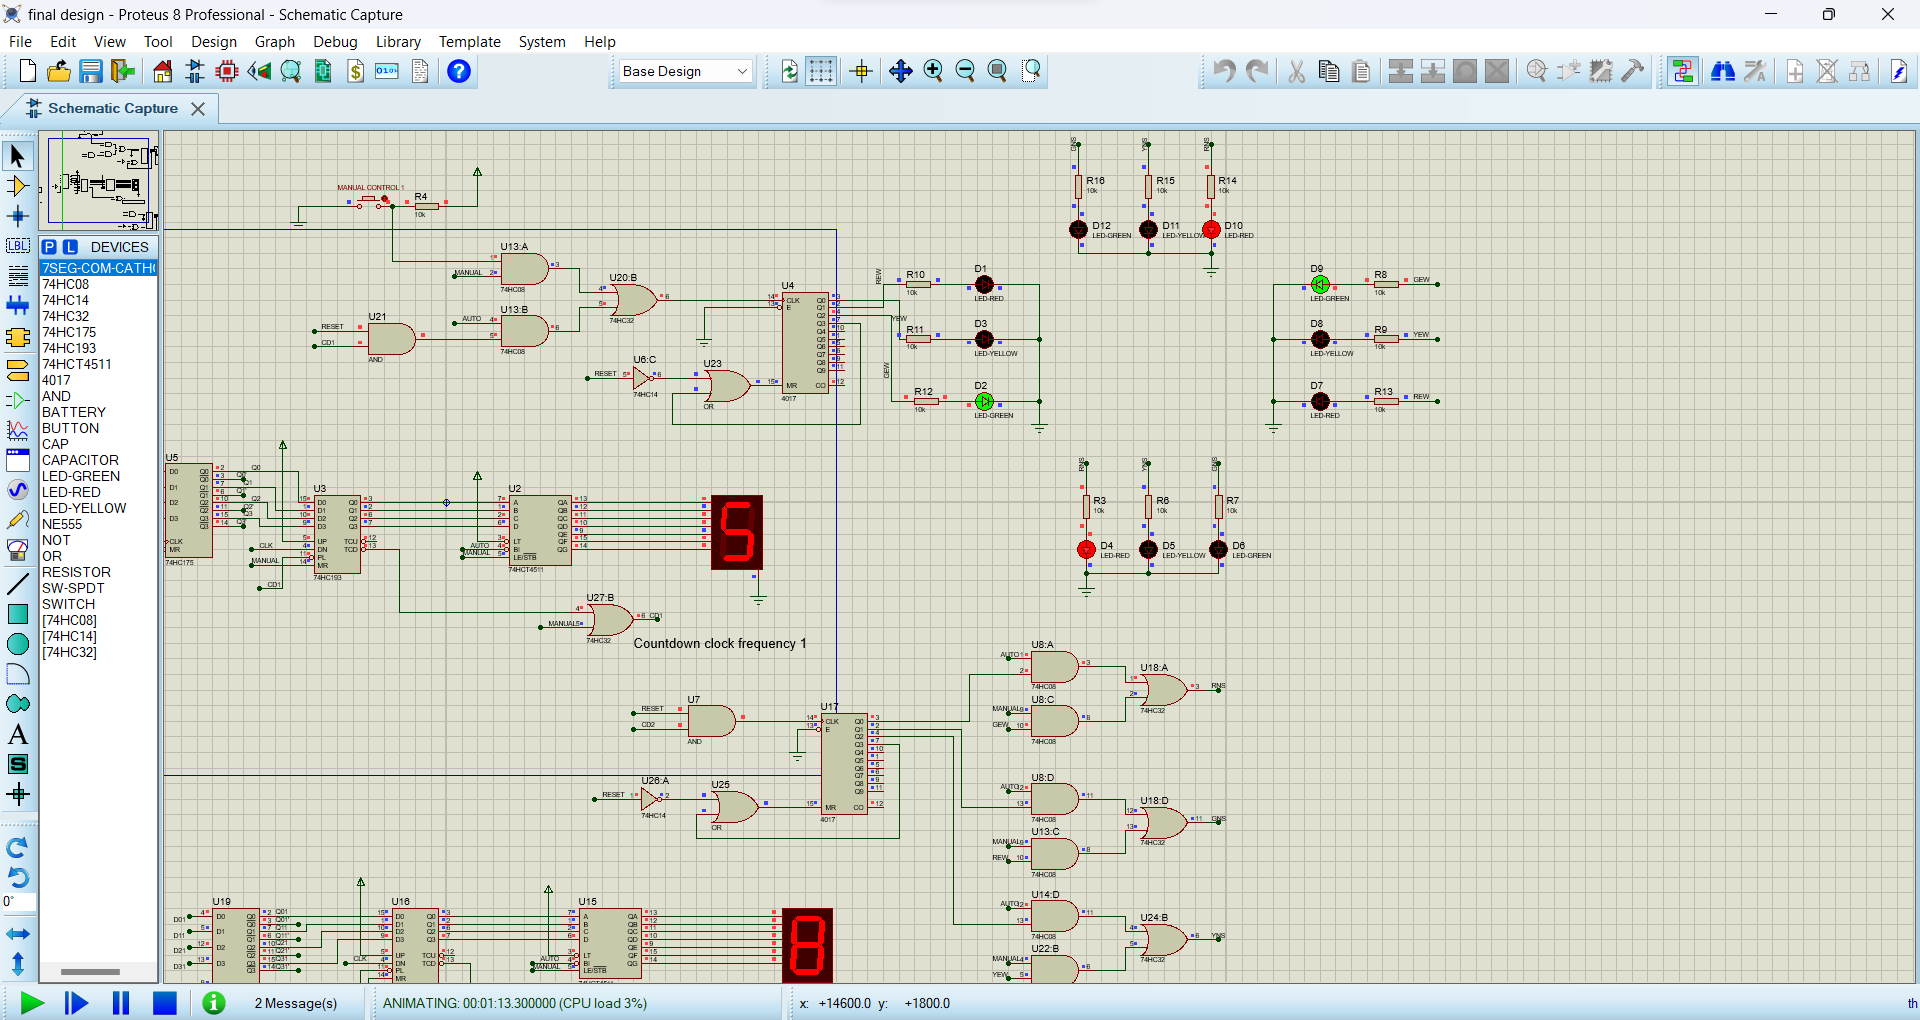
\includegraphics[width=14cm]{Pic/Proteus/Automatic_2.png}
    \caption{State GREEN-RED.}
    \label{fig:enter-label}
\end{figure}

\begin{figure}[h]
    \centering
    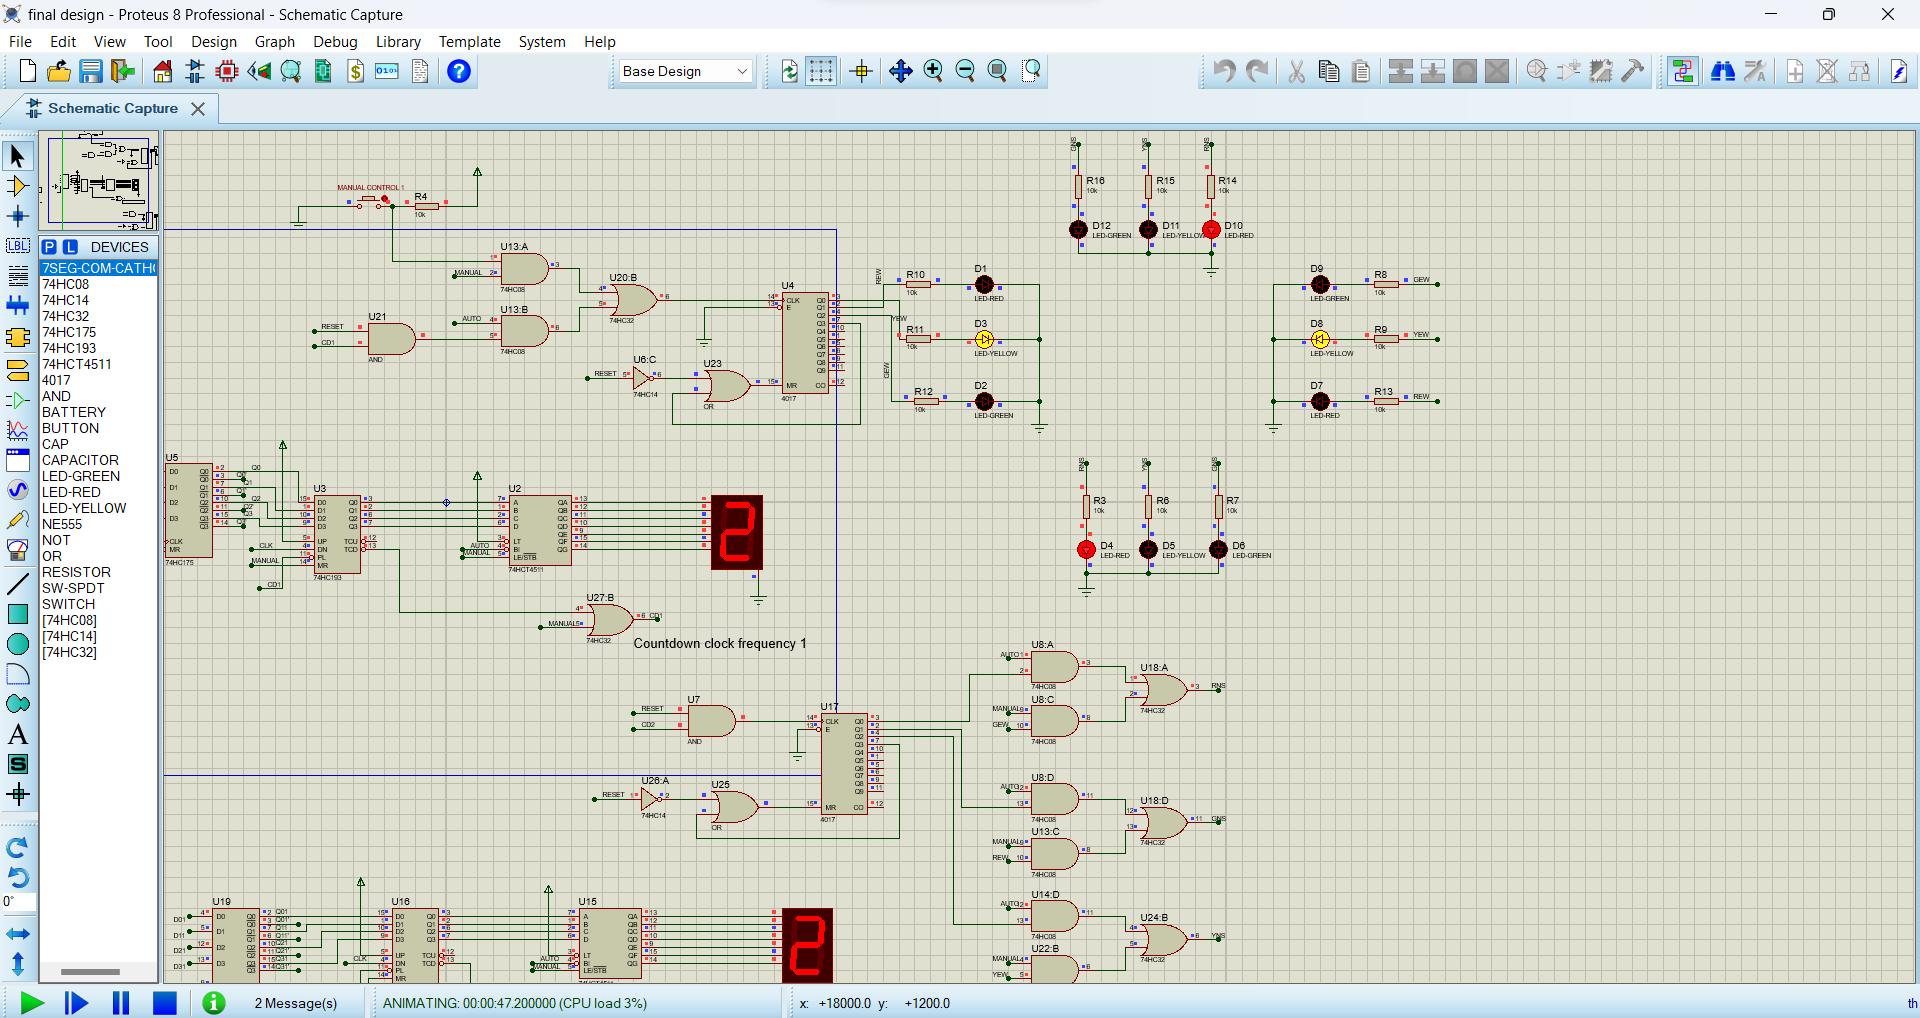
\includegraphics[width=14cm]{Pic/Proteus/Automatic_3.png}
    \caption{State YELLOW-RED.}
    \label{fig:enter-label}
\end{figure}

In summary, the Automatic Mode work correctly as our group expected. Next is to check the \textbf{Manual Mode} of the project. In this mode, there will be three different states. They are RED-GREEN, YELLOW-YELLOW and GREEN-RED. Here are the output of our simulation on Proteus:\par
\newpage
\begin{figure}[h]
    \centering
    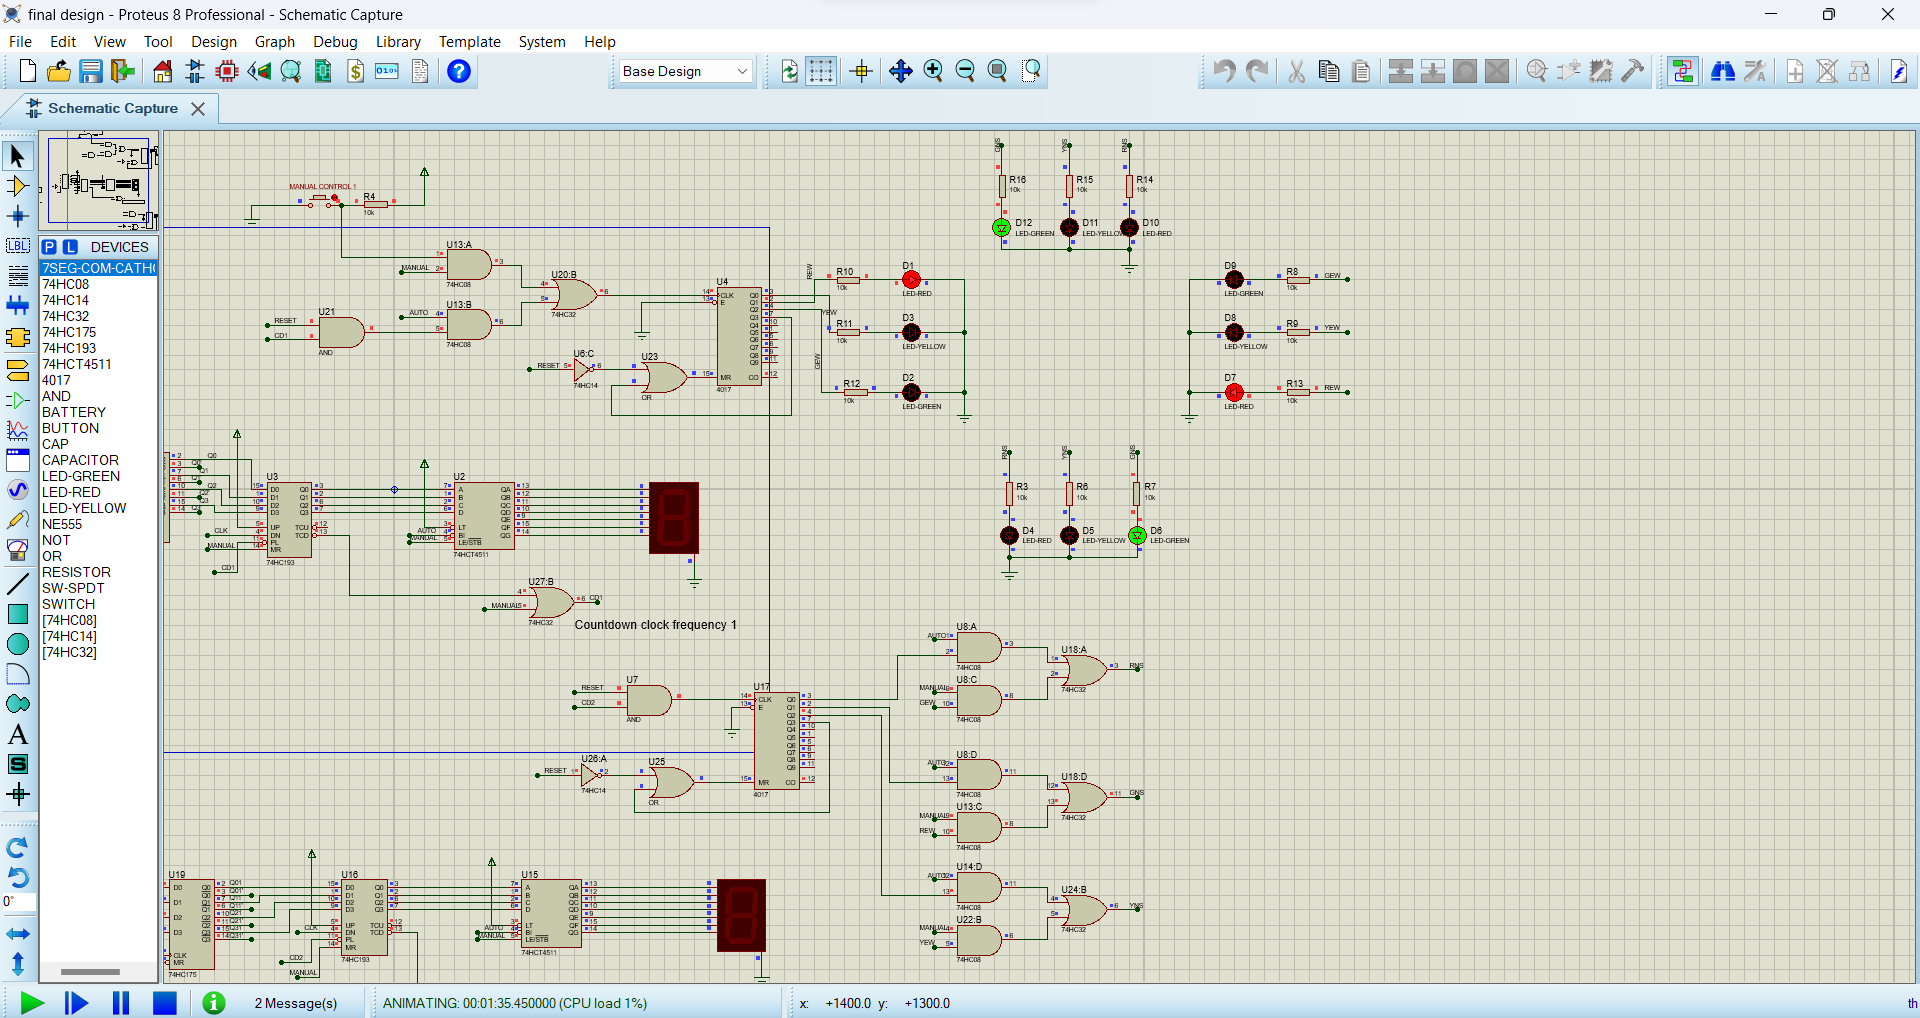
\includegraphics[width=14cm]{Pic/Proteus/Manual_0.png}
    \caption{State: RED-GREEN.}
    \label{fig:enter-label}
\end{figure}

\begin{figure}[h]
    \centering
    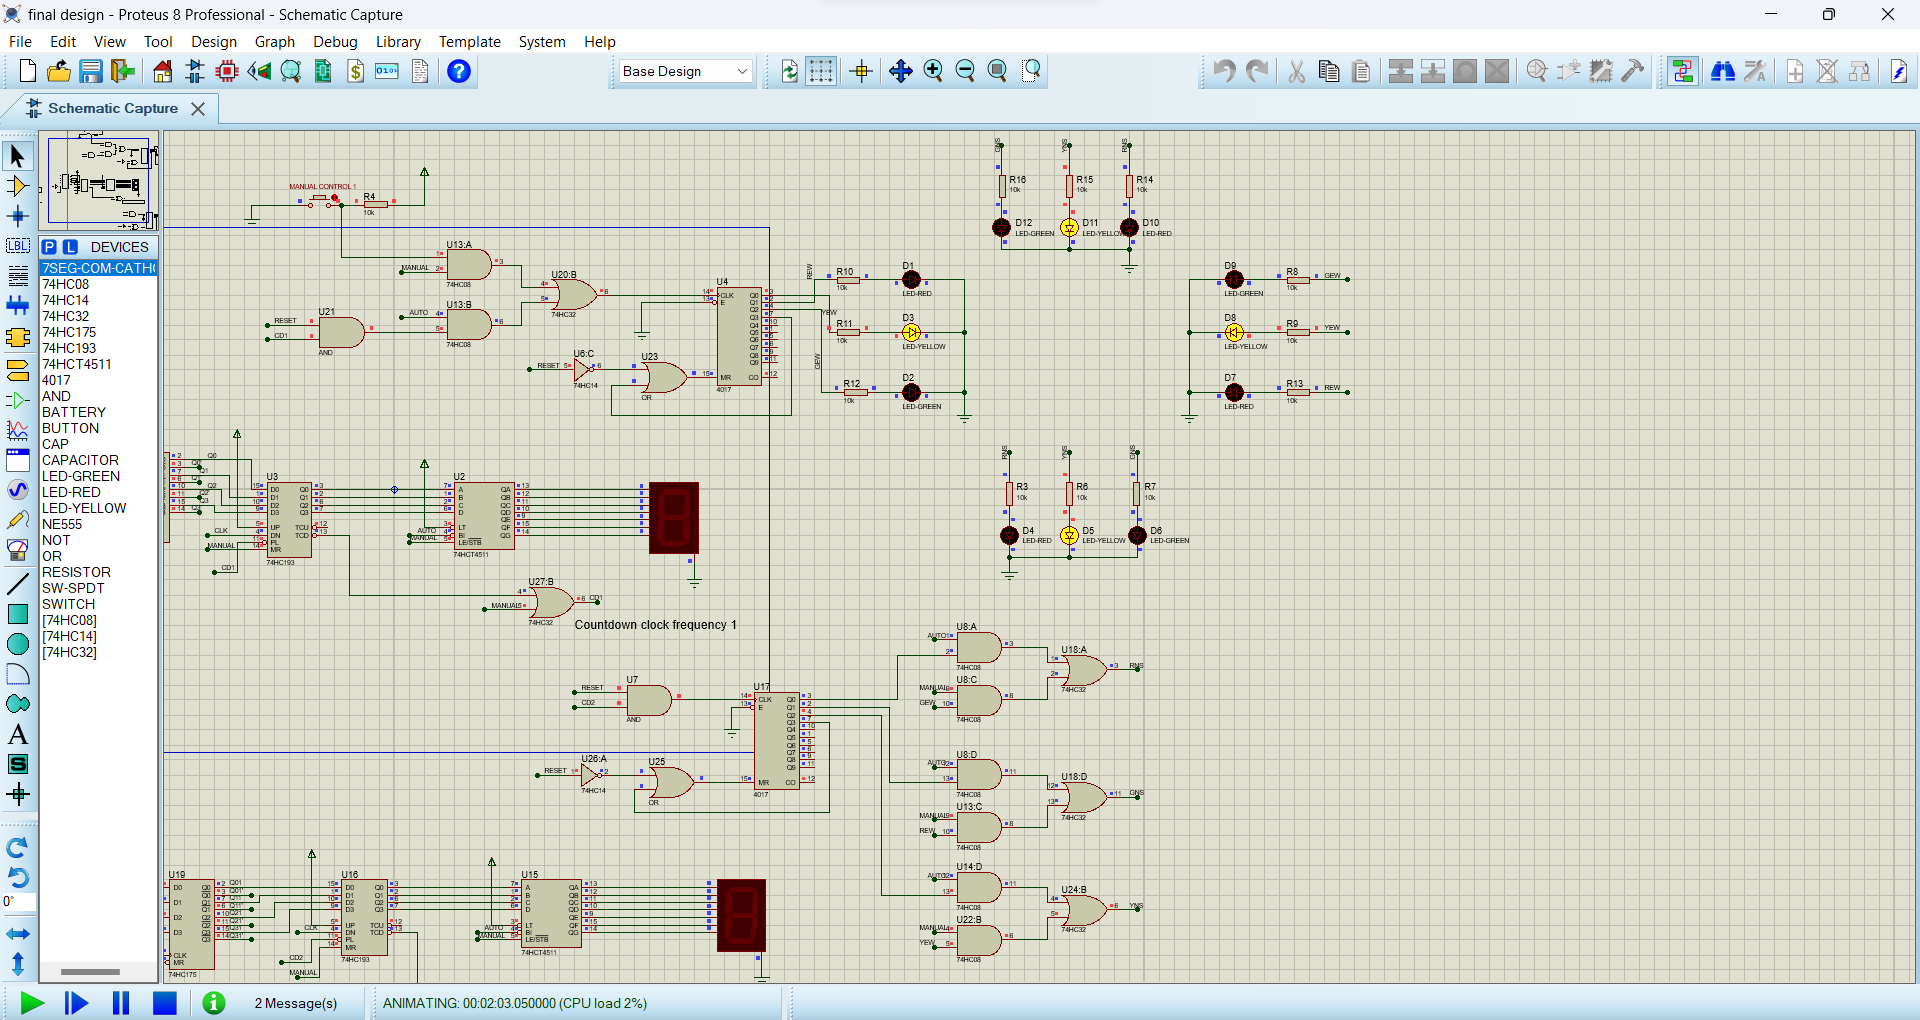
\includegraphics[width=14cm]{Pic/Proteus/Manual_1.png}
    \caption{State: YELLOW-YELLOW.}
    \label{fig:enter-label}
\end{figure}

\newpage
\begin{figure}[h]
    \centering
    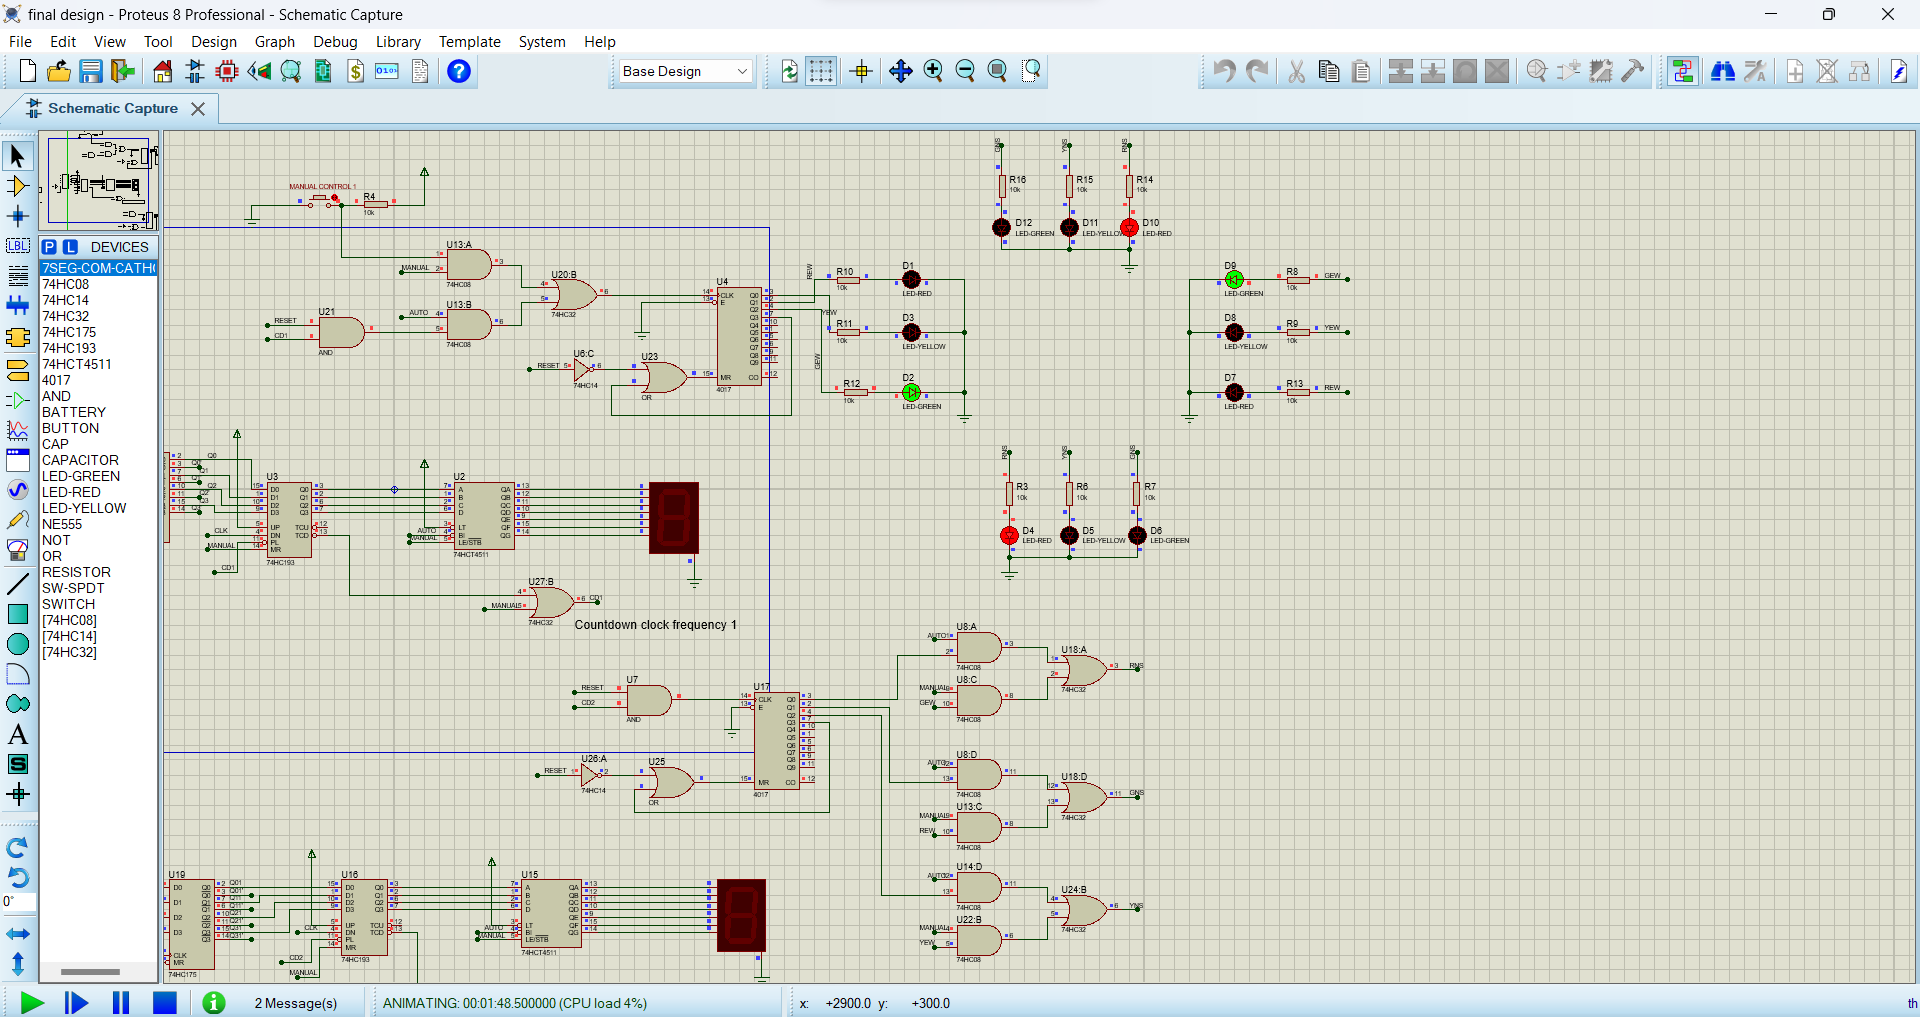
\includegraphics[width=14cm]{Pic/Proteus/Manual_2.png}
    \caption{State: GREEN-RED.}
    \label{fig:enter-label}
\end{figure}


In the end, our simulation not only met but exceeded our expectations. The designed scenario unfolded just as we had envisioned, underscoring the success of our planning and execution. Every aspect of the simulation fell neatly into place, affirming a smooth and accurate representation of our initial projections.\par

\newpage
\subsection{Real Life Implementation}
\begin{figure}[h]
    \centering
    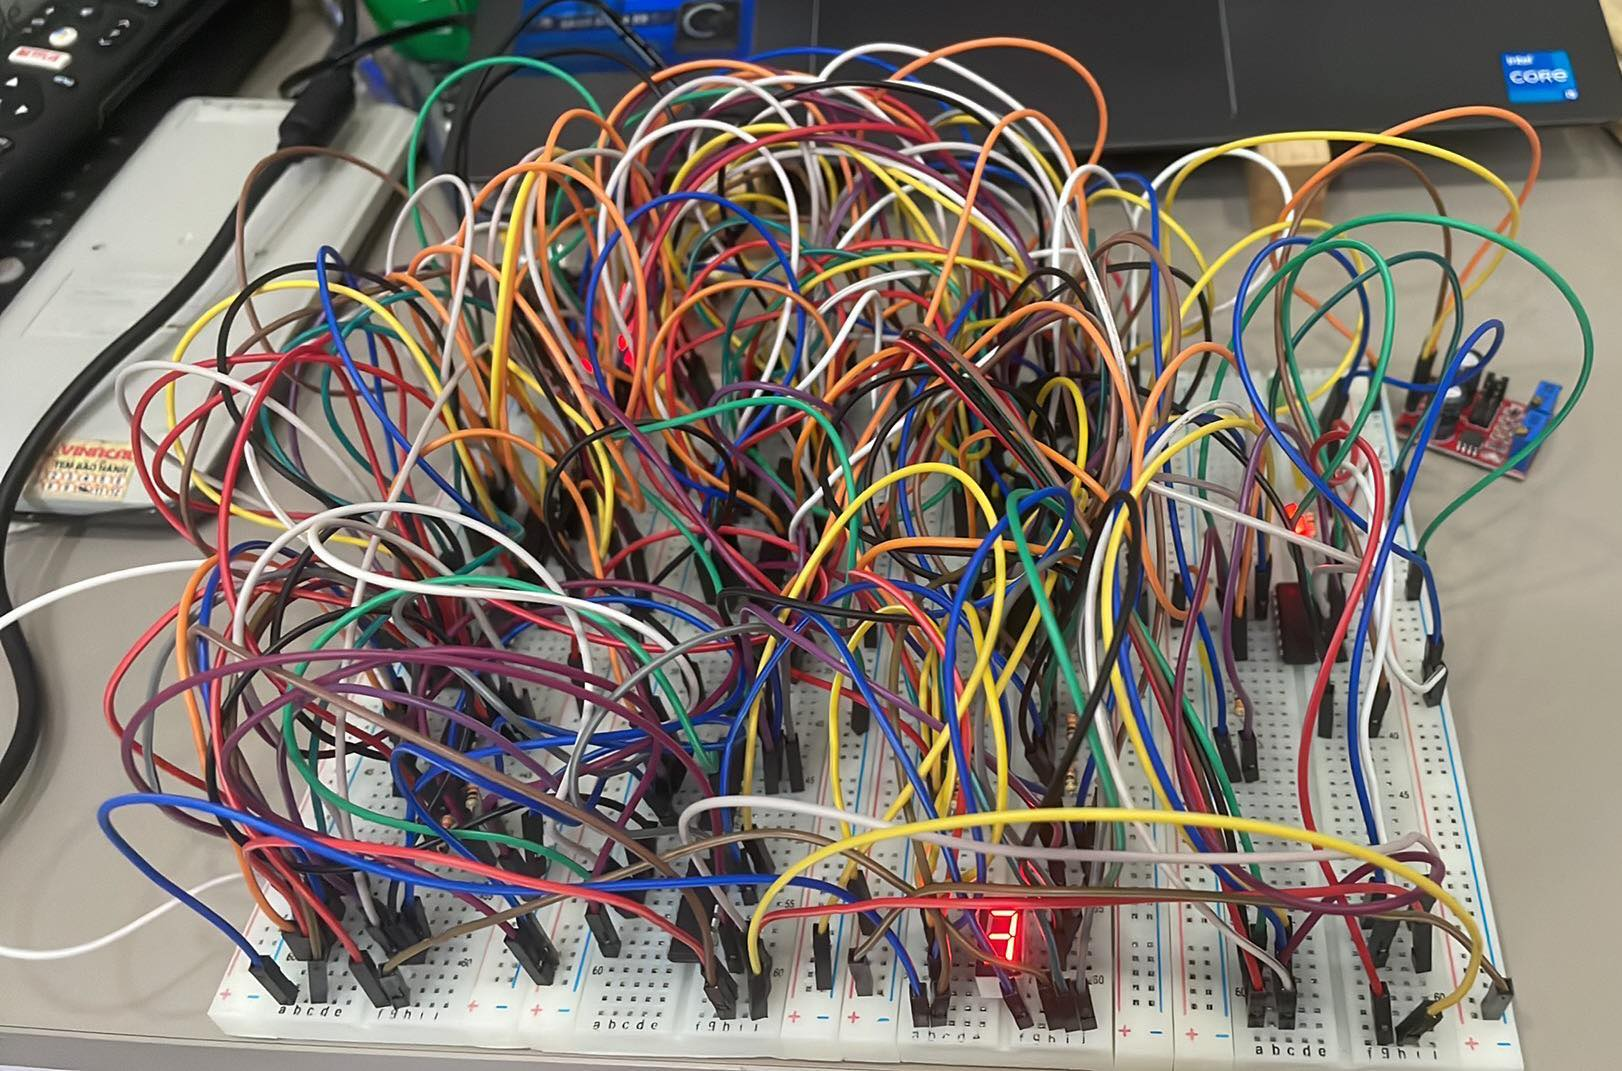
\includegraphics[width=12cm]{Pic/Proteus/real life imp.jpg}
    \caption{Real life implementation.}
    \label{fig:enter-label}
\end{figure}

\begin{figure}[h]
    \centering
    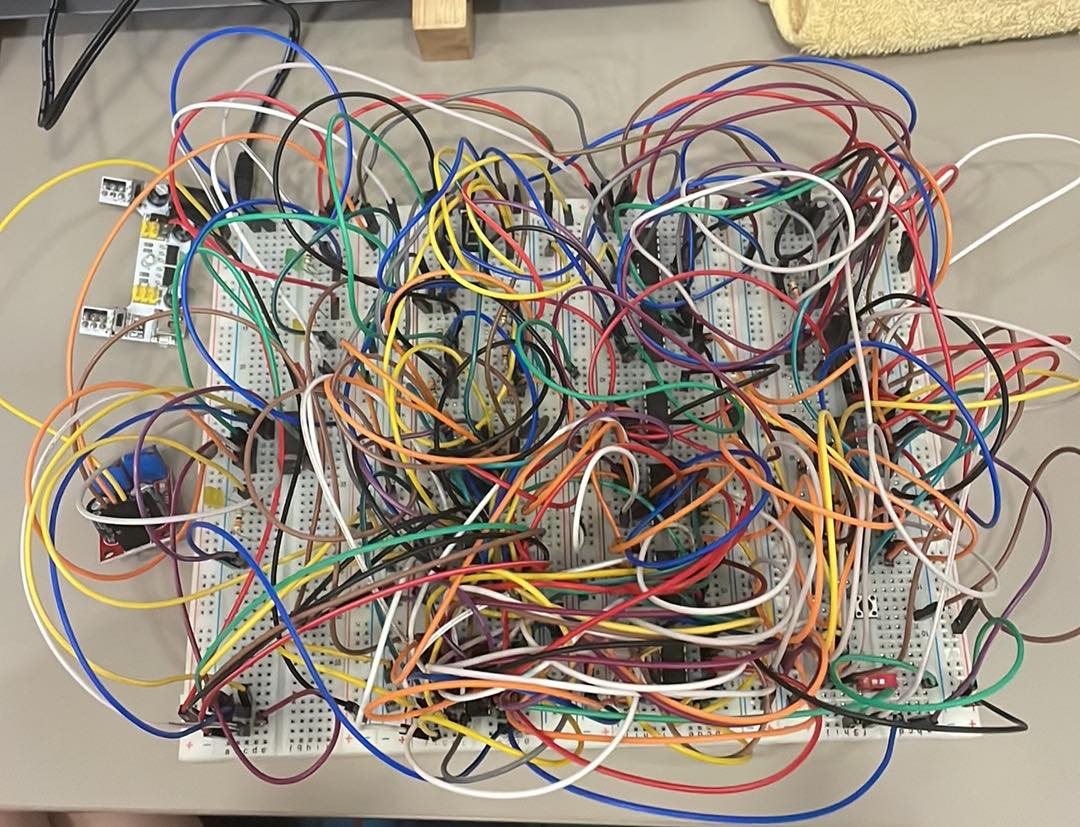
\includegraphics[width=12cm]{Pic/Proteus/real life imp 2.jpg}
    \caption{Real life implementation.}
    \label{fig:enter-label}
\end{figure}

Here is the link to the video of implementation: \href{https://drive.google.com/file/d/1nSew7hscdaEV-AUZaBXrrWRVpo7kgrah/view?usp=sharing}{Video}
\newpage

\section{Summary}
In this project, our group successfully implemented a four-way traffic control system using only logic design principles. The primary goal was to create an efficient and reliable traffic management system without the need for complex components. Leveraging the capabilities of specific integrated circuits (ICs), such as SN74LS175N, SN74LS193N, and CD4511BE, our group designed a robust control mechanism.\par\vspace{5pt}

The system operates in two modes: Automatic and Manual. In Automatic Mode, the traffic signals follow a predefined sequence, ensuring smooth traffic flow based on set durations. Meanwhile, Manual Mode provides flexibility for manual intervention, allowing authorities to manage traffic situations such as jams effectively.\par\vspace{5pt}

To enhance the system's functionality, our group incorporated a 7-segment display to visually represent the countdown sequence. This display, driven by CD4017BE, accurately reflects the changing signal states, providing a clear indication of the traffic pattern.\par\vspace{5pt}

The successful simulation demonstrated the seamless integration of logic design principles, IC functionalities, and manual control features. This project not only showcases the practical application of logic circuits in traffic management but also serves as a testament to the effectiveness of our design and implementation.\par\vspace{5pt}

If you have any question about the project, cotact us via: \url{nam.nguyenolkmphy@hcmut.edu.vn}\par\vspace{5pt}
Here are the link to access our simulation on Proteus: \href{https://github.com/knammm/Logic-Design-Project}{GitHub}.\par
\newpage

\bibliographystyle{plain}
% \bibliography{refs}
\begin{thebibliography}{90}
\bibitem{} Dejan, 555 Timer IC – Working Principle, Block Diagram, Circuit Schematics, \url{https://howtomechatronics.com/how-it-works/555-timer-ic-working-principle-block-diagram-circuit-schematics/}
\bibitem{} Øyvind Nydal Dahl, How Does a 555 Timer Work?, \url{https://www.build-electronic-circuits.com/how-does-a-555-timer-work/#:~:text=The%20555%20timer%20works%20by,resets%20a%20flip%2Dflop%20accordingly.}
\bibitem{} MECSU, IC đếm CD4017, \url{https://mecsu.vn/ho-tro-ky-thuat/tim-hieu-ic-dem-cd4017.bKy#:~:text=CD4017%20l%C3%A0%20vi%20m%E1%BA%A1ch%20%C4%91%E1%BA%BFm,c%E1%BA%A1nh%20d%C6%B0%C6%A1ng%20c%E1%BB%A7a%20xung%20clock.}
\bibitem{} IC CD4511, \url{https://dientutuonglai.com/cd4511.html}
\bibitem{} MECSU, Sơ đồ chân bộ đếm nhị phân 4 bit 74LS93, \url{https://mecsu.vn/ho-tro-ky-thuat/tim-hieu-so-do-chan-bo-dem-nhi-phan-4-bit-74ls93.O4L}

\end{thebibliography}

\newpage

\nocite{*}
\end{document}
